\documentclass[12pt, openany]{article}

\usepackage{import}
\usepackage{config}

\usepackage{xcolor}
\usepackage{makeidx}
\usepackage{multicol}

\usepackage[]{caption}

\usepackage[sorting=none]{biblatex}

\addbibresource{biblio.bib}
\renewcommand*{\bibfont}{\small}
%\setlength{\bibitemsep}{0pt} % Pas d'espace entre les références


%{\fontsize{10pt}{14pt}\selectfont}
%{\scriptsize}





\begin{document}
\lstset{inputencoding=utf8/latin1}
\renewcommand{\labelitemi}{$\bullet$}

\begin{titlepage}
  \begin{sffamily}
  \begin{center}

    
\includegraphics[width=0.9\linewidth]{logo.png}~\\[0.5cm]

    %\textsc{ds\LARGE }\\[2cm]

    \textsc{\Large Discrete Mathematics \\ Project - Group 3}\\[1.5cm]


    \color{centrale_red}\HRule \\[0cm]
    { \huge \bfseries \color{centrale_red} \textit{Optimization techniques}\\ Graph-based optimization for resource allocation during an outbreak\\ }

    \HRule \\[0.5cm]

    {\Large \bfseries \color{centrale_red} -- Final report -- }
    \color{black}
    %\includegraphics[width=0.8\textwidth]{CM/granta/moduleYoung_coursIDM.png}
    %\begin{center}
     %    Les différentes familles de matériaux illustrées par leur module d'Young\\(Source : \cite{diapoIDMcha1})
    %\end{center}
    %\\%[2cm]

    \vspace{2.5cm}

    \begin{minipage}{0.4\textwidth}
      \begin{flushleft} \large
      \textit{\textbf{Students}} \\[0.5cm]
      Szymon \textsc{Cichy, 235 093}\\
    Maxime \textsc{Luce}, 294 620 \\

  
      \end{flushleft}
    \end{minipage}
    \begin{minipage}{0.4\textwidth}
      \begin{flushright} \large
      \textit{\textbf{Teacher}} \\[0.5cm]
       Marcin \textsc{Bodych}\\
      \end{flushright}
    \end{minipage}

    \vfill


    {Academic year 2025/2026 -- 12th June 2026}

  \end{center}
  \end{sffamily}
\end{titlepage}

\clearpage % end title page

%\begingroup
%  \pagestyle{empty}
%  \null
%  \newpage
%\endgroup

\tableofcontents

\newpage

\addcontentsline{toc}{section}{Problem Overview and Motivation}
\section*{Problem Overview and Motivation}

During a health crisis such as an epidemic, the rapid distribution of critical resources (e.g., vaccines, medical staff, intensive care beds) is a matter of survival. But the logistics infrastructure (roads, plains, and so on) has limited capacities and might be subject to road closures.

This project aims to model this logistical challenge as an optimization problem on a directed network and graph. Our objectives are to design, implement, and analyze algorithms capable of computing the maximum allocation of resources in real time in all possible scenarios.

\section{General overview of flow networks and optimization}

\subsection{Flow networks and common definitions}

In order to explain the \emph{maximum flow} problem, we must introduce the \emph{flow network}.

\begin{figure}[H]
\centering
\begin{tikzpicture}[
    scale=1.2,
    >=stealth,
    vertex/.style={circle, draw, minimum size=11mm, inner sep=0pt},
    flow/.style={-{Stealth[length=3mm]}, thick},
    edge/.style={thick}
]

% Nodes
\node[vertex] (s) at (0,1.5) {$s$};
\node[vertex] (a) at (2.8,3.0) {$a$};
\node[vertex] (b) at (2.8,0.0) {$b$};
\node[vertex] (c) at (6.0,3.0) {$c$};
\node[vertex] (d) at (6.0,0.0) {$d$};
\node[vertex] (t) at (8.8,1.5) {$t$};
% Solid edges
\draw[flow] (s) -- node[midway, above] {$\frac{3}{5}$} (a);
\draw[flow] (s) -- node[midway, below] {$\frac{2}{2}$} (b);
\draw[flow] (a) -- node[midway, left] {$\frac{1}{2}$} (b);
\draw[flow] (a) -- node[midway, below] {$\frac{2}{3}$} (c);
\draw[flow] (b) -- node[midway, below] {$\frac{3}{4}$} (d);
\draw[flow] (c) -- node[midway, left] {$\frac{1}{1}$} (d);
\draw[flow] (c) -- node[midway, above] {$\frac{1}{2}$} (t);
\draw[flow] (d) -- node[midway, below] {$\frac{4}{5}$} (t);
\end{tikzpicture}
\caption{Example flow network}
\end{figure}



\begin{definition}[Flow Network]
A directed graph representing transport of flow between nodes. This directed graph can be written as $G = (V,E)$ where \(V\) is the set of vertices, \(E \subseteq V \times V\) is the set of directed edges, \(s \in V\) is the source, \(t \in V\) is the sink and \(c : E \to \mathbb{R}_{\ge 0}\) is the capacity function.
\end{definition}

\begin{definition}[Capacity function]
    Description

    \[
        \forall (u,v) \in E :
        \begin{cases}
        c(v,u) = 0, & \text{if } (v,u) \notin E
        \end{cases}
    \]
\end{definition}

\begin{definition}[Edge Capacity]
The maximum amount of flow that an edge can carry.
\end{definition}

\begin{definition}[Flow]
Quantity transmitted through an edge, limited by its \emph{capacity}.
\end{definition}

\begin{definition}[Node (Vertex)]
A point in the network where flow can enter or leave.
\end{definition}

\begin{definition}[Arc (Edge)]
A directed connection between two \emph{nodes}.
\end{definition}

\begin{definition}[Source]
A node with only outgoing flow.
\end{definition}

\begin{definition}[Sink]
A node with only incoming flow.
\end{definition}

\begin{definition}[Flow function]
Description
    \[
f : E \to \mathbb{R}_{\ge 0}
\]
such that it follows the \emph{capacity constraint} and the \emph{flow conservation}.
\end{definition}

\begin{definition}[Capacity constraint]
The capacity constraint states that we cannot exceed the capacity of each edge.
\[
    0 \le f(u,v) \le c(u,v)
    \qquad \forall (u,v)\in E
    \]
\end{definition}

\begin{definition}[Flow conservation / Kirchhoff's Law]
The Kirchhoff's law states that for any node $k \in V \backslash \{s,t\}$, the sum of incoming flows equals the sum of outgoing flows:
\[
    \sum_{(u,v)\in E} f(u,v)
    \;=\;
    \sum_{(v,w)\in E} f(v,w)
    \qquad \forall v \in V \setminus \{s,t\}
    \]
\end{definition}

\begin{definition}[Excess Function]
Excess Function derived from \textbf{flow conservation}. It represents the difference between the total incoming and outgoing flow at vertex \(v\). For a flow network \(G = (V,E)\) with flow \(f\), the excess function of a vertex \(v\) is defined as

\[
e(v) =
\sum_{(u,v)\in E} f(u,v)
-
\sum_{(v,w)\in E} f(v,w)
\]
\end{definition}





\begin{itemize}

\item \textbf{Conserving} vertex \(e(v) = 0\): Flow into the vertex equals flow leaving it.
\item \textbf{Active} vertex \(e(v) > 0\) indicating excess incoming flow. \textbf{Sink} \(t\) is active
\item \textbf{Deficient} vertex \(e(v) < 0\) indicating more outgoing than incoming flow. \textbf{Source} \(s\) is deficient


\end{itemize}
The value of a \textbf{feasible flow} (or just \textbf{flow}) for a network is the net flow into the sink \(t\):
\[
-e(s) = |f| = e(t)
\]


\subsection{Max-Flow Min-Cut Theorem}

The main theorem for flow networks is the \emph{Max-Flow Min-Cut Theorem} that states that the maximal flow that can go through the network is exactly equal to the capacity of the minimal cut.


\begin{figure}[H]
\centering
\begin{tikzpicture}[
    scale=1.2,
    >=stealth,
    % Styles des noeuds
    vertex/.style={circle, draw, minimum size=11mm, inner sep=0pt},
    sourcepart/.style={fill=blue!15}, % Couleur pour la partition S
    sinkpart/.style={fill=red!15},    % Couleur pour la partition T
    % Styles des arêtes et de la coupe
    flow/.style={-{Stealth[length=3mm]}, thick},
    cutline/.style={dashed, red, ultra thick}
]

% Nodes - Partition S (Source)
\node[vertex, sourcepart] (s) at (0,1.5) {$s$};
\node[vertex, sourcepart] (a) at (2.8,3.0) {$a$};
\node[vertex, sourcepart] (b) at (2.8,0.0) {$b$};

% Nodes - Partition T (Sink)
\node[vertex, sinkpart] (c) at (6.0,3.0) {$c$};
\node[vertex, sinkpart] (d) at (6.0,0.0) {$d$};
\node[vertex, sinkpart] (t) at (8.8,1.5) {$t$};

% Solid edges (flots originaux conservés)
\draw[flow] (s) -- node[midway, above] {$\frac{3}{5}$} (a);
\draw[flow] (s) -- node[midway, below] {$\frac{2}{2}$} (b);
\draw[flow] (a) -- node[midway, left] {$\frac{1}{2}$} (b);
\draw[flow] (a) -- node[midway, below] {$\frac{2}{3}$} (c);
\draw[flow] (b) -- node[midway, below] {$\frac{3}{4}$} (d);
\draw[flow] (c) -- node[midway, left] {$\frac{1}{1}$} (d);
\draw[flow] (c) -- node[midway, above] {$\frac{1}{2}$} (t);
\draw[flow] (d) -- node[midway, below] {$\frac{4}{5}$} (t);

% min cut
\draw[cutline] (4.4, 3.8) to[out=270, in=90] (4.4, -0.8) 
    node[below, text=black, font=\bfseries] {Min-Cut (Capacity = $4+3 = 7$)};

\node[vertex, sourcepart, minimum size=5mm] at (1.5, -1.8) {};
\node[right] at (1.8, -1.8) {Partition $S$ (max $3$)};

\node[vertex, sinkpart, minimum size=5mm] at (5.5, -1.8) {};
\node[right] at (5.8, -1.8) {Partition $T$ (max $4$)};

\end{tikzpicture}
\caption{Flow network illustrating the partitioning for the Min-Cut}
\end{figure}

In order to solve the maximum flow problem, several algorithms were proposed and run mostly in polynomial time and give optimal solutions as summarized in \tableref{alg_max_min_cut}.

\begin{table}[H]
\centering
\begin{tabular}{|l|c|l|}
\hline
\textbf{Algorithm} & \textbf{Year} & \textbf{Time Complexity} \\
\hline
Ford--Fulkerson & 1956 & $O(E \cdot |f^*|)$ \\
Edmonds--Karp & 1969 & $O(VE^2)$ \\
Dinic's Algorithm & 1970 & $O(V^2E)$ \\
Push--Relabel & 1986 & $O(V^3)$ \\
\hline
\end{tabular}
\caption{Algorithms for solving the Maximum Flow problem}
\label{tab:alg_max_min_cut}
\end{table}

\subsection{Lagrange multiplier}

In section \ref{sec:lagrangian_kkt}, we will use the Lagrangian to present and use the Karush–Kuhn–Tucker (KKT) conditions.

We seek in this part to determine the extrema of a function $f : \mathscr{U} \subset E \to \mathbb{R}$ of class $\mathscr{C}^1$ subject to the constraint $g(x)=0$, where $g$ is itself a real-valued function of class $\mathscr{C}^1$ on $\mathscr{U}$.

To determine $\underset{g(x)=0}{\min} f(x)$, a naive approach consists of deriving from the constraint $g(x_1, \dots, x_n)=0$ a relation of the form $x_n = \varphi(x_1, \dots, x_{n-1})$. We thereby reduce the problem to the optimization techniques of the previous section:

$$ \min_{g(x)=0} f(x) = \min_{(x_1, \dots, x_{n-1}) \in \mathscr{U}'} f(x_1, \dots, x_{n-1}, \varphi(x_1, \dots, x_{n-1})) $$

where $\mathscr{U}'$ would be a subset of $E$ to be specified.

Nevertheless, even if specific results justify, under the condition $\mathrm{d}g_x \neq 0$, the possibility of expressing one of the variables as a function of the others, the proposed approach proves in practice to be quickly ineffective: one does not generally have an explicit expression and the latter is often only valid locally.

\vspace{10pt}

\noindent\begin{minipage}{.52\linewidth}
The mathematician Joseph-Louis Lagrange proposed another approach, based on the following geometric point of view. Let us consider the function $f$ defined on $\mathbb{R}^2$ by $f(x, y) = x^2 + y^2$ and a constraint of the form $g(x, y) = 0$ where $g : \mathbb{R}^2 \to \mathbb{R}$ is assumed to be of class $\mathscr{C}^1$. $f$ reaches a (global) minimum at $(0,0)$ but this differs from $\underset{g(x,y)=0}{\min} f(x, y)$ if $g(0,0) \neq 0$.

\vspace{10pt}

As illustrated by the graph opposite, when $f$ has a minimum at $M_0 = (x_0, y_0)$ under the constraint $g(x_0, y_0) = 0$, the level curve relating to $f$ at $M_0$ is tangent to the curve with equation $g(x, y) = 0$. In other words, the two gradients $\nabla f(M_0)$ and $\nabla g(M_0)$ are collinear: $\nabla f(M_0) = \lambda \nabla g(M_0)$. 

The ratio $\lambda$ is called the \textit{Lagrange multiplier}.
\end{minipage}
\hfill
\begin{minipage}{.45\linewidth}
    \centering
    
\includegraphics[width=\linewidth]{img/lagrange_muliplier.png}
    (Source: \cite{cours_prost})
\end{minipage}

\subsubsection{Definitions and core theorem}

In order to make this section easier to read, we present in this subsection the basic of the Lagrange multiplier, based on \cite{cours_prost}. First, we need to define the \emph{differential}.

\begin{definition}[Differential at a point]

    A map $f : \mathscr{U} \subset E \to F$ is said to be differentiable at $a \in \mathscr{U}$ if there exists $\varphi \in \mathscr{L}(E, F)$ such that:
    $$f(a+h) \underset{h \to 0_E}{=} f(a) + \varphi(h) + o(\|h\|)$$
    
    If the map $\varphi$ exists, it is unique and is then called the \textit{differential} of $f$ at the point $a$, but also the \textit{tangent linear map} to $f$ at $a$. It is denoted by $\mathrm{d}f_a$ or $\mathrm{d}f(a)$.
\end{definition}

Then, we can present the \emph{Lagrange multiplier theorem} (in the case of a single constraint).

\begin{theorem}[Lagrange multiplier]
    Let $f$ and $g$ be two real-valued functions of class $\mathscr{C}^1$ on the \textbf{open set} $\mathscr{U}$ of $E$ and $X = \{x \in \mathscr{U} \mid g(x) = 0\}$.
    
    If the restriction of $f$ to $X$ has a local extremum at $a \in X$ and $\mathrm{d}g_a \neq 0$, then $\mathrm{d}f_a$ is collinear with $\mathrm{d}g_a$.
\end{theorem}

\subsubsection{Example of finding the minimum of a function}

Let us determine $\underset{x^2+y^2=1}{\min} x y$ by setting $f(x, y) = x y$ and $g(x, y) = x^2 + y^2 - 1$. (source: \cite{cours_prost})

\begin{itemize}
    \item The two real-valued functions $f$ and $g$ are polynomial and therefore of class $\mathscr{C}^\infty$ on the open set $\mathbb{R}^2$.
    \item The unit circle $X = \{(x, y) \in \mathbb{R}^2 \mid g(x, y) = 0\}$ being compact, $f_{|X}$ has a minimum at $(x_0, y_0) \in X$.
    \item $\nabla f(x, y) = \begin{bmatrix} y \\ x \end{bmatrix}$ and $\nabla g(x, y) = 2\begin{bmatrix} x \\ y \end{bmatrix} \neq 0$ for all $(x, y) \in X$. From the above, there exists $\lambda \in \mathbb{R}^*$ such that:


$$
\begin{cases}
y_0 = 2\lambda x_0 \\
x_0 = 2\lambda y_0 \\
x_0^2 + y_0^2 = 1
\end{cases}
$$

We find $(x_0, y_0, \lambda) = \left(\pm \frac{1}{\sqrt{2}}, \pm \frac{1}{\sqrt{2}}, \frac{1}{2}\right)$ or else $(x_0, y_0, \lambda) = \left(\pm \frac{1}{\sqrt{2}}, \mp \frac{1}{\sqrt{2}}, -\frac{1}{2}\right)$.

Hence $\boxed{\underset{x^2+y^2=1}{\min} x y = -\frac{1}{2}}$.

\end{itemize}

\begin{figure}[H]
    \centering
    
\includegraphics[width=0.9\linewidth]{img/min_xy_sphere_unite.png}
    \caption{Illustration of the minimum of the function $f(x, y) = x y$ under the constraint $g(x, y) = x^2 + y^2 - 1$ to determine $\underset{x^2+y^2=1}{\min} x y$.}
    \label{fig:min_xy_sphere_unite}
\end{figure}

\subsubsection{Volume and surface area of a box}

We wish to manufacture a box in the shape of a rectangular parallelepiped, without a top cover. The volume of this box must be equal to $0.5 \;\meter^3$ and to optimize the amount of material used, we want the sum of the areas of the faces to be as small as possible. What dimensions should we choose to manufacture the box? (source: \cite{bibmath_extrema_exo18})


\begin{itemize}
    \item Let $x, y,$ and $z$ be the three dimensions of the box (with $x, y, z > 0$, where $x$ and $y$ are the dimensions of the base, and $z$ is the height).

    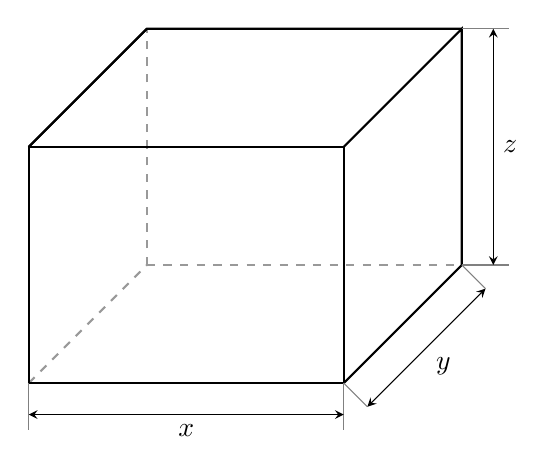
\begin{tikzpicture}[scale=1]

    % Définition des coordonnées des sommets de la boîte
    \coordinate (O) at (0,0);       % Avant gauche bas
    \coordinate (A) at (4,0);       % Avant droite bas
    \coordinate (B) at (4,3);       % Avant droite haut
    \coordinate (C) at (0,3);       % Avant gauche haut
    \coordinate (D) at (1.5,1.5);   % Arrière gauche bas
    \coordinate (E) at (5.5,1.5);   % Arrière droite bas
    \coordinate (F) at (5.5,4.5);   % Arrière droite haut
    \coordinate (G) at (1.5,4.5);   % Arrière gauche haut

    % Tracé des arêtes cachées (en pointillés)
    \draw[thick, dashed, gray!80] (O) -- (D);
    \draw[thick, dashed, gray!80] (D) -- (E);
    \draw[thick, dashed, gray!80] (D) -- (G);

    % Tracé des arêtes visibles
    \draw[thick] (O) -- (A) -- (B) -- (C) -- cycle; % Face avant
    \draw[thick] (A) -- (E) -- (F) -- (B);          % Face droite
    \draw[thick] (C) -- (G) -- (F);                 % Face supérieure (partie)
    \draw[thick] (G) -- (C);                        % Arête avant-gauche (déjà tracée par cycle, mais pour la propreté)
    \draw[thick] (G) -- (F);                        % Arête arrière-haute

    % --- Lignes de cote et flèches ---

    % Dimension x (base, largeur)
    \draw[thin, gray] (O) -- (0,-0.6);
    \draw[thin, gray] (A) -- (4,-0.6);
    \draw[<->, >=stealth] (0,-0.4) -- (4,-0.4) node[midway, below] {$x$};

    % Dimension y (base, profondeur)
    \draw[thin, gray] (A) -- (4.3,-0.3);
    \draw[thin, gray] (E) -- (5.8,1.2);
    \draw[<->, >=stealth] (4.3,-0.3) -- (5.8,1.2) node[midway, below right] {$y$};

    % Dimension z (hauteur)
    \draw[thin, gray] (E) -- (6.1,1.5);
    \draw[thin, gray] (F) -- (6.1,4.5);
    \draw[<->, >=stealth] (5.9,1.5) -- (5.9,4.5) node[midway, right] {$z$};

\end{tikzpicture}
    
    Its volume is $V(x,y,z) = xyz = 0.5$.
    
    We want to minimize the surface area function:
    $$f(x, y, z) = xy + 2xz + 2yz$$
    (we have removed the top face).

    \item Finding the critical point using Lagrange Multipliers
    
    The functions $f$ and $V$ are of class $\mathcal{C}^1$ on the open set $U = (0, +\infty)^3$. We are looking for the extrema of $f$ subject to the constraint $V(x,y,z) = 0.5$.

    The gradient of $V$ is $\nabla V = (yz, xz, xy)$, which is never zero on $U$. 
    
    According to the Lagrange multipliers theorem, if $f$ has a local extremum under this constraint, there exists a real number $\lambda$ such that $\nabla f(x, y, z) = \lambda \nabla V(x, y, z)$. 
    This yields the following system of equations:
    \begin{equation}
    \begin{cases}
        \pdv{f}{x} = \lambda \pdv{V}{x} \implies y + 2z = \lambda yz \\[1.5ex]
        \pdv{f}{y} = \lambda \pdv{V}{y} \implies x + 2z = \lambda xz \\[1.5ex]
        \pdv{f}{z} = \lambda \pdv{V}{z} \implies 2x + 2y = \lambda xy \\[1.5ex]
        xyz = 0.5
    \end{cases}
    \end{equation}
    
    To solve this system, we can multiply the first three equations by $x$, $y$, and $z$ respectively:
    \begin{equation*}
    \begin{cases}
        xy + 2xz = \lambda xyz \\
        xy + 2yz = \lambda xyz \\
        2xz + 2yz = \lambda xyz
    \end{cases}
    \end{equation*}

    Equating the right-hand sides of the first two equations, we get:
    $$xy + 2xz = xy + 2yz \implies 2xz = 2yz$$
    Since $z > 0$, we deduce that $x = y$. 
    
    Substituting $x = y$ into the second and third equations gives:
    $$x^2 + 2xz = 4xz \implies x^2 = 2xz$$
    Since $x > 0$, we deduce that $x = 2z$. 
    
    We now have $x = y = 2z$. Substituting these into the volume constraint $xyz = 0.5$:
    $$(2z)(2z)z = 0.5 \implies 4z^3 = 0.5 \implies z^3 = \frac{1}{8} \implies z = \frac{1}{2}$$
    From this, we find $x = 2\left(\frac{1}{2}\right) = 1$ and $y = 2\left(\frac{1}{2}\right) = 1$.
    The only critical point is therefore $(1, 1, 1/2)$.

    \item Proving it is a global minimum
    
    It remains to be proven that this critical point indeed corresponds to a global minimum. To do this, we can substitute $z = \frac{1}{2xy}$ (from the volume constraint) into the area function, which leads us to seek the minimum of the two-variable function:
    $$g(x,y) = xy + \frac{1}{x} + \frac{1}{y}$$
    on the open set $U' = ]0, +\infty[ \times ]0, +\infty[$. 
    The critical point $(1,1,1/2)$ for $f$ corresponds to the critical point $(1,1)$ for $g$.
    
    We notice that $g(1, 1) = 3$. 
    Furthermore, if $x < 1/3$ or $y < 1/3$, then $g(x,y) > 3 = g(1,1)$. We can deduce that:
    $$\inf\{g(x,y) \mid (x,y) \in U'\} = \inf\{g(x,y) \mid (x,y) \in A\}$$
    where $A = \{(x,y) \in \mathbb{R}^2 \mid x \ge 1/3 \text{ and } y \ge 1/3\}$. 
    
    But moreover, if $(x,y) \in A$ satisfies $x > 3$ or $y > 3$, then $g(x,y) \ge 3 = g(1,1)$. We deduce that:
    $$\inf\{g(x,y) \mid (x,y) \in U'\} = \inf\{g(x,y) \mid (x,y) \in K\}$$
    where $K = [1/3, 3] \times [1/3, 3]$. 
    
    Now, $K$ is compact and $g$ is continuous on $K$, so we know that $g$ admits a global minimum on $K$. This minimum on $K$ is also the minimum of $g$ on $U'$. 
    However, $g$ can only admit a minimum at a critical point. Thus $g$ admits a minimum at $(1, 1)$. 
    
    This means that the three dimensions minimizing the surface area are \boxed{x = 1, y = 1, $ and $z = 1/2}.
\end{itemize}

\begin{figure}[H]
    \centering
    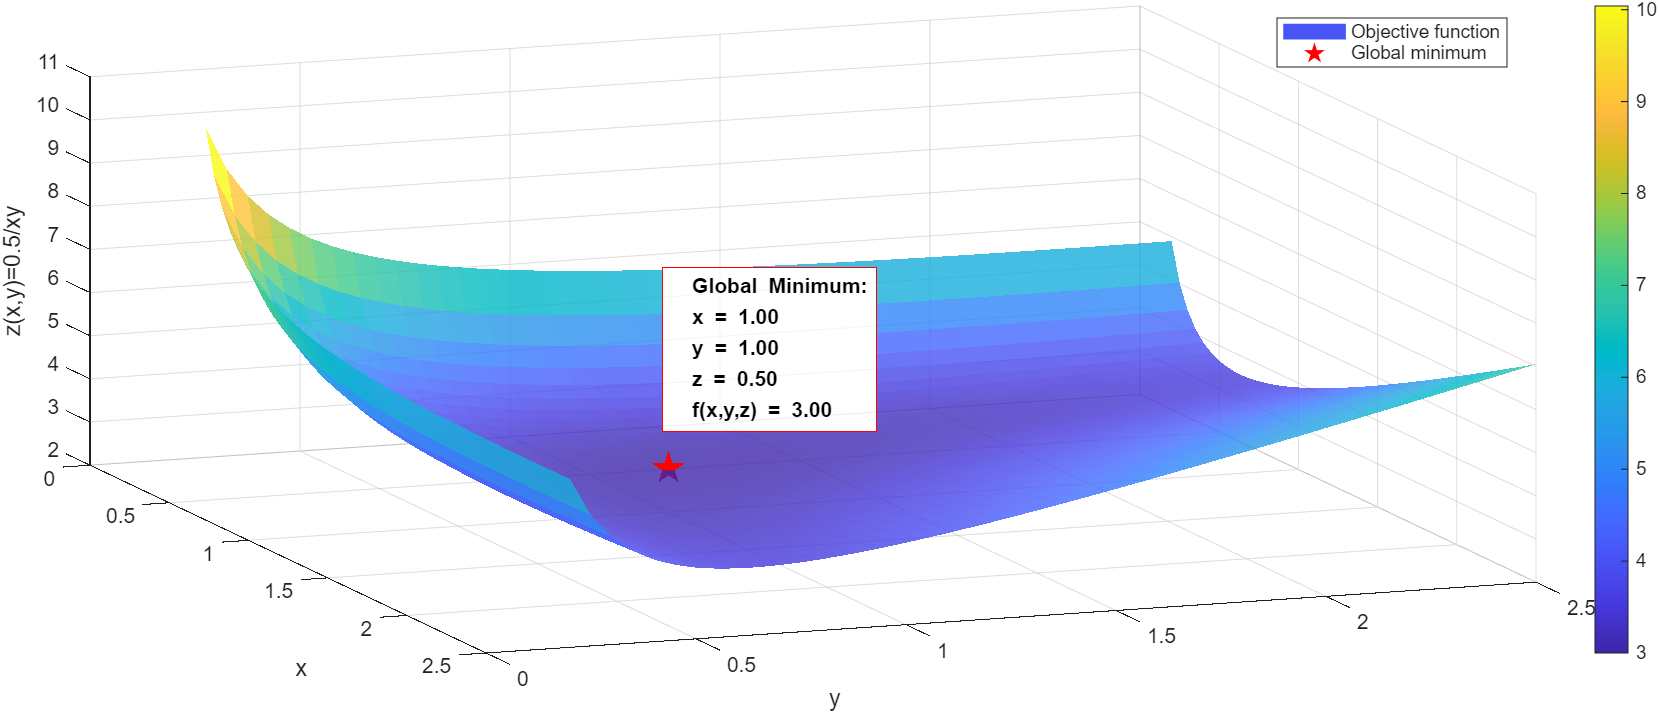
\includegraphics[width=\linewidth]{Project/img/min_surface_volume.png}
    \caption{Illustration of the solving of $\underset{xyz=0.5}{\min} xy+2xz+2yz$ on a local domain space.}
    \label{fig:placeholder}
\end{figure}

\subsubsection{Lagrange Multipliers}
There is an extension of the previous theorem for $p$ constraints that is as follows:

\begin{theorem}[Lagrange Multipliers]
    Let $f$ and $g_1, \dots, g_p$ be real-valued functions of class $\mathscr{C}^1$ on the \textbf{open set} $\mathscr{U}$ of $E$ and:
    $$X = \{x \in \mathscr{U} \mid g_1(x) = \dots = g_p(x) = 0\}$$
    
    If the restriction of $f$ to $X$ has a local extremum at $a \in X$ and if the linear forms $\mathrm{d}g_{1,a}, \dots, \mathrm{d}g_{p,a}$ are independent, then there exist $\lambda_1, \dots, \lambda_p \in \mathbb{R}$ such that $\mathrm{d}f_a = \lambda_1 \mathrm{d}g_{1,a} + \dots + \lambda_p \mathrm{d}g_{p,a}$.
    
    The real numbers $\lambda_1, \dots, \lambda_p$ are called \textit{Lagrange multipliers}.
\end{theorem}

\newpage
\section{Flow networks, duality, fairness}
\subsection{NetworX library and algorithmic approach}

We use the \texttt{import networkx as nx} python library to define flow network graphs in Python. The flow network is built manually as a \texttt{nx.DiGraph} directed graph from an array of tuples.

\begin{minted}[linenos, bgcolor=bg]{python}
G = nx.DiGraph()

arcs = [
    ("s", "a", 8),
...
    ("d", "t", 8),
]

for u, v, capacity in arcs:
    G.add_edge(u, v, capacity=capacity)
def hello():
    print("Hello")
\end{minted}

Without implementing flow algorithms themselves, we can then use various \texttt{NetworkX} methods to solve the basic problem.
\begin{minted}[linenos, bgcolor=bg]{python}
# default using preflow_push()
flow_value, flow_dict = nx.max_flow(G, s_source, t_sink)
# S, T are partitions after cut
cut_value, (S, T) = nx.min_cut(G, s_source, t_sink)

# we can also use specific algorithms to obtain
# a residual flow graph R without building it manually
R = nx.algorithms.flow.edmonds_karp(G, s_source, t_sink)
flow_dict = nx.algorithms.flow.build_flow_dict(G, R)
\end{minted}

Finally, we can plot the flow networks using \texttt{import matplotlib as plt} library, with the help of \texttt{networkx} own \texttt{matplotlib}-based helpers

\begin{minted}[linenos, bgcolor=bg]{python}
fig, ax = plt.subplots(...)

nx.draw_networkx_nodes(G, pos, nodelist, ...)
nx.draw_networkx_edges(G, pos, edgelist, ...)
nx.draw_networkx_labels(...)
nx.draw_networkx_edge_labels(...)

...

plt.show()
\end{minted}

The important insight this approach provides is that the solution for both \textit{max network flow} and \textit{max-flow min-cut} problems is obtained not only by the same algorithm, but a single algorithm pass provides the solution for both by the way of residual graph. When using algorithmic approach, this graph allows us to obtain graph partitions using BFS search, by defining non-reachable nodes as those with no residual capacity

\begin{minted}[linenos, bgcolor=bg]{python}
S = set()
q = deque(["s"])
S.add("s")
while q:
    u = q.popleft()
    for v in R.successors(u):
        residual_capacity = capacity[(u, v)] - flow[(u, v)]
        if v not in S and residual_capacity > 0:
            S.add(v)
            q.append(v)
      
min_cut = [(u, v) for u, v in G.edges() if u in S and v not in S]
T = set(G.nodes()) - S
\end{minted}

\begin{figure}[H]
    \centering
    \begin{subfigure}{.49\linewidth}
        \centering
        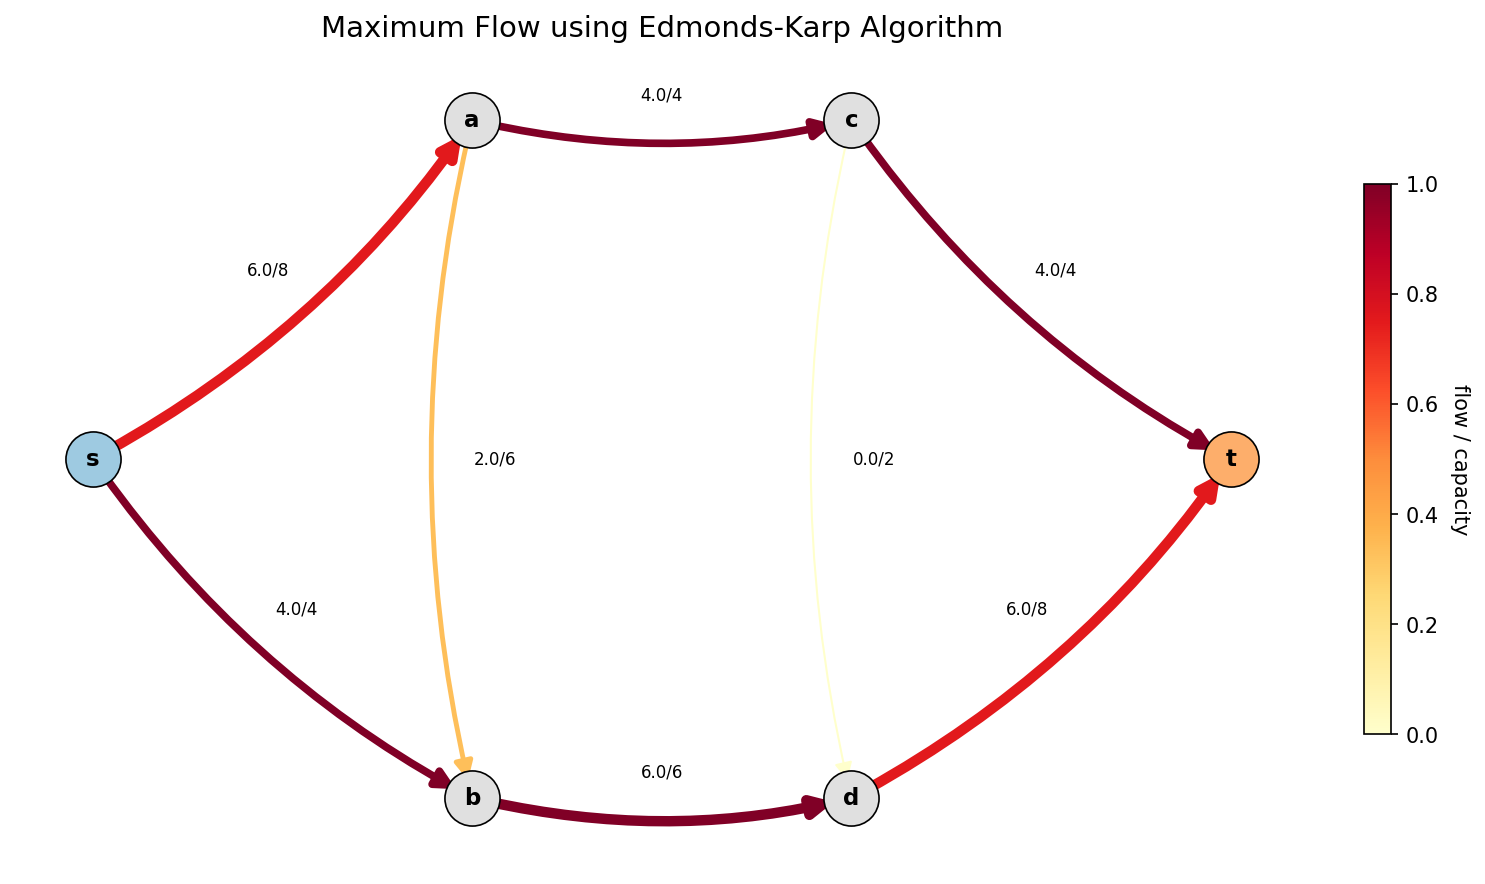
\includegraphics[width=\linewidth]{Project/img/edmonds_karp_max_flow.png}
        \caption{}
        \label{fig:edmonds_karp_max_flow}
    \end{subfigure}
    \begin{subfigure}{.49\linewidth}
        \centering
        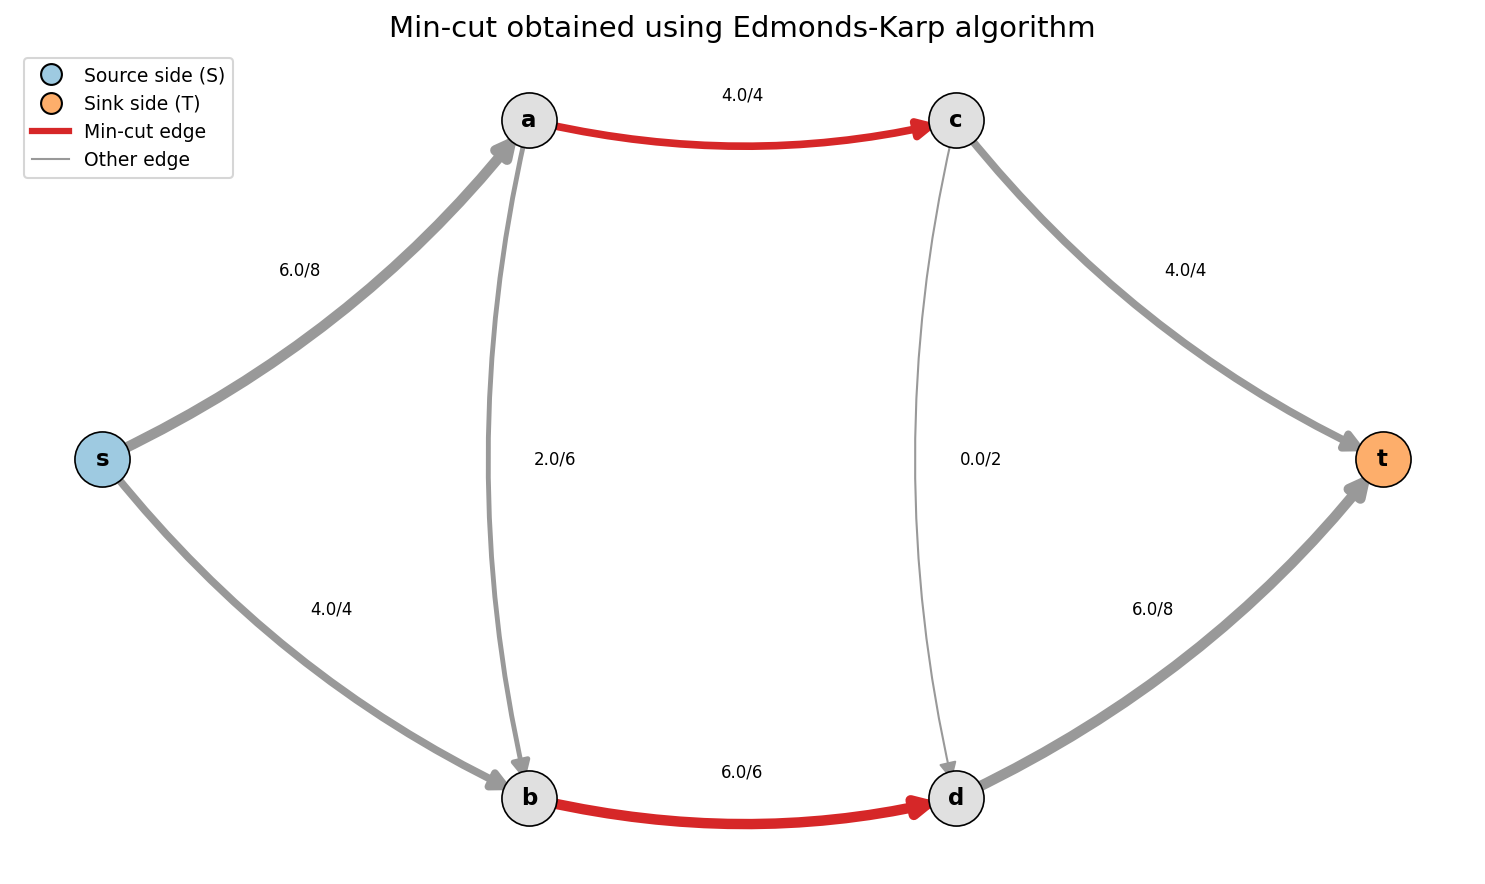
\includegraphics[width=\linewidth]{Project/img/edmonds_karp_min_cut.png}
        \caption{}
        \label{fig:edmonds_karp_min_cut}
    \end{subfigure}
    \caption{\textbf{Results of Edmonds-Karp algorithm.} The \figref{edmonds_karp_max_flow} presents edge utility saturation (\texttt{flow / capacity}. \figref{edmonds_karp_min_cut} highlights node sets and edges in a min-cut obtained using BFS search on a residual flow graph.}
    \label{fig:edmonds_karp}
\end{figure}

\subsection{Convex optimization and Linear programming formulation}

Linear programming is an optimization method that allows us to obtain a best outcome, defined by a \textit{linear objective function}, constrained by a set of \textit{linear equality and inequality constraints} that form a \textit{feasible region}. This region is geometrically represented by a convex polytope, formed by a set of half-space intersections in the $\mathbb{R}^n$ space ($n$ representing the dimensions of the objective vector). The objective vector $x$ is a vector of \textit{decision variables}, which the linear program calculates. It is a point in the feasible region that represents an optimal solution $f(x^*) = f^* = OPT$. There can be many optimal solutions.

To begin with, we will redefine the max network flow problem in terms of a set of linear equations, using matrix notation.


We start with the following optimization problem:
\[
\begin{aligned}
\text{maximize} \quad & f = q^\top x \\[4pt]
\text{subject to} \quad
& Ax = 0, \\[4pt]
& 0 \le x \le c .
\end{aligned}
\]

Let the flow variables be collected in the vector
\[
x=
\begin{bmatrix}
f(e_1)\\
f(e_2)\\
\vdots\\
f(e_m)
\end{bmatrix}
\in\mathbb{R}^m,
\]
where \(m=|E|\). Thus, \(x\) is the vector of edge flows.

The vector
\[
q \in \mathbb{R}^m
\]
selects the flow leaving the source \(s\), and is defined by
\[
q_i =
\begin{cases}
1, & \text{if } e_i=(s,v)\in E, \\[4pt]
-1, & \text{if } e_i=(v,s)\in E, \\[4pt]
0, & \text{otherwise.}
\end{cases}
\]

Hence, \(q^\top x\) equals the net flow leaving the source \(s\). By flow conservation, this is also equal to the net flow entering the sink \(t\).

The capacity vector is
\[
c \in \mathbb{R}_{\ge 0}^m,
\]
where \(c_i\) is the capacity of edge \(e_i\).

Let \(n=|V|\). The matrix
\[
A \in \mathbb{R}^{(n-2)\times m}
\]
is the reduced node-edge incidence matrix, obtained by removing the rows corresponding to the source \(s\) and sink \(t\). Its entries are defined by
\[
A_{u,i} =
\begin{cases}
1 & \text{if edge } e_i=(u,v), \\
-1 & \text{if edge } e_i=(v,u), \\
0 & \text{otherwise,}
\end{cases}
\qquad u \in V\setminus\{s,t\}.
\]

Finally, we can obtain the array representation of the problem for use in \texttt{cvxpy} library

\begin{minted}[linenos, bgcolor=bg]{python}
incidence_mx = np.asarray(nx.incidence_matrix(G, oriented=True).todense())
A = incidence_mx[1:-1, :]
c = np.array([d['capacity'] for (_, _, d) in G.edges(data=True)])
x = cvxpy.Variable(len(G.edges()), nonneg=True)
q = np.array([1 if u == "s" else -1 if v == "s" else 0 for u, v in G.edges()])

# Objective function f = q @ x
f = cvxpy.Maximize(q @ x)
problem = cvxpy.Problem(f, c)
problem.solve()
\end{minted}

Thus, we have obtained a solution to the max network flow problem. Before showing the results and comparing them to the algorithmic method, let us discuss the other side of this problem - max-flow min-cut. In the previous example, we have obtained a residual graph that contained a solution for both, but because our Linear Programming approach is problem-agnostic: the optimizer does not know that it is solving a graph problem, only that it is finding a vector constrained by a set of equations.

Therefore, in order to solve the max-flow min-cut problem, we have to define another set of variables, constraints and objectives.

\[
\begin{aligned}
\text{minimize} \quad & d^\top c \\[4pt]
\text{subject to} \quad
& d_{uv} - z_u + z_v \ge 0,
    && \forall(u,v)\in E,\ u\ne s,\ v\ne t, \\[4pt]
& d_{sv} + z_v \ge 1,
    && \forall(s,v)\in E,\ v\ne t, \\[4pt]
& d_{ut} - z_u \ge 0,
    && \forall(u,t)\in E,\ u\ne s, \\[4pt]
& d_{st} \ge 1,
    && \forall(s,t)\in E, \\[4pt]
\text{sign const.} \quad
& d_{uv} \ge 0 \quad \forall(u,v) \in V\\[4pt]
& z_u \in \mathbb{R} \quad \forall(u) \in E \setminus \{s, t\}
\end{aligned}
\]

\begin{figure}[H]
    \centering
    \begin{subfigure}{.49\linewidth}
        \centering
        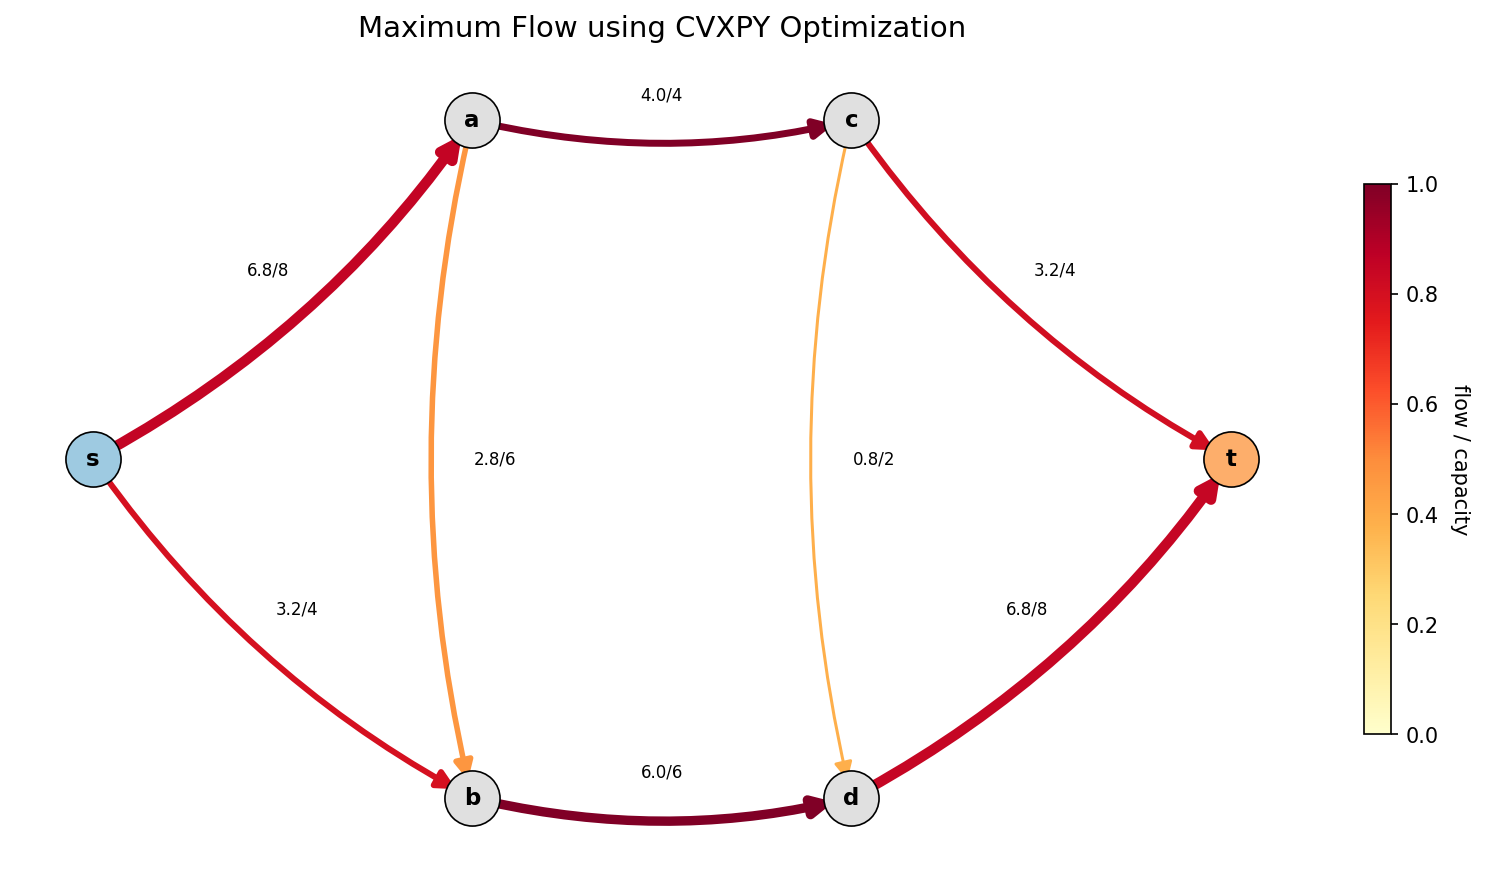
\includegraphics[width=\linewidth]{Project/img/cvxpy_max_flow.png}
        \caption{}
        \label{fig:cvxpy_max_flow}
    \end{subfigure}
    \begin{subfigure}{.49\linewidth}
        \centering
        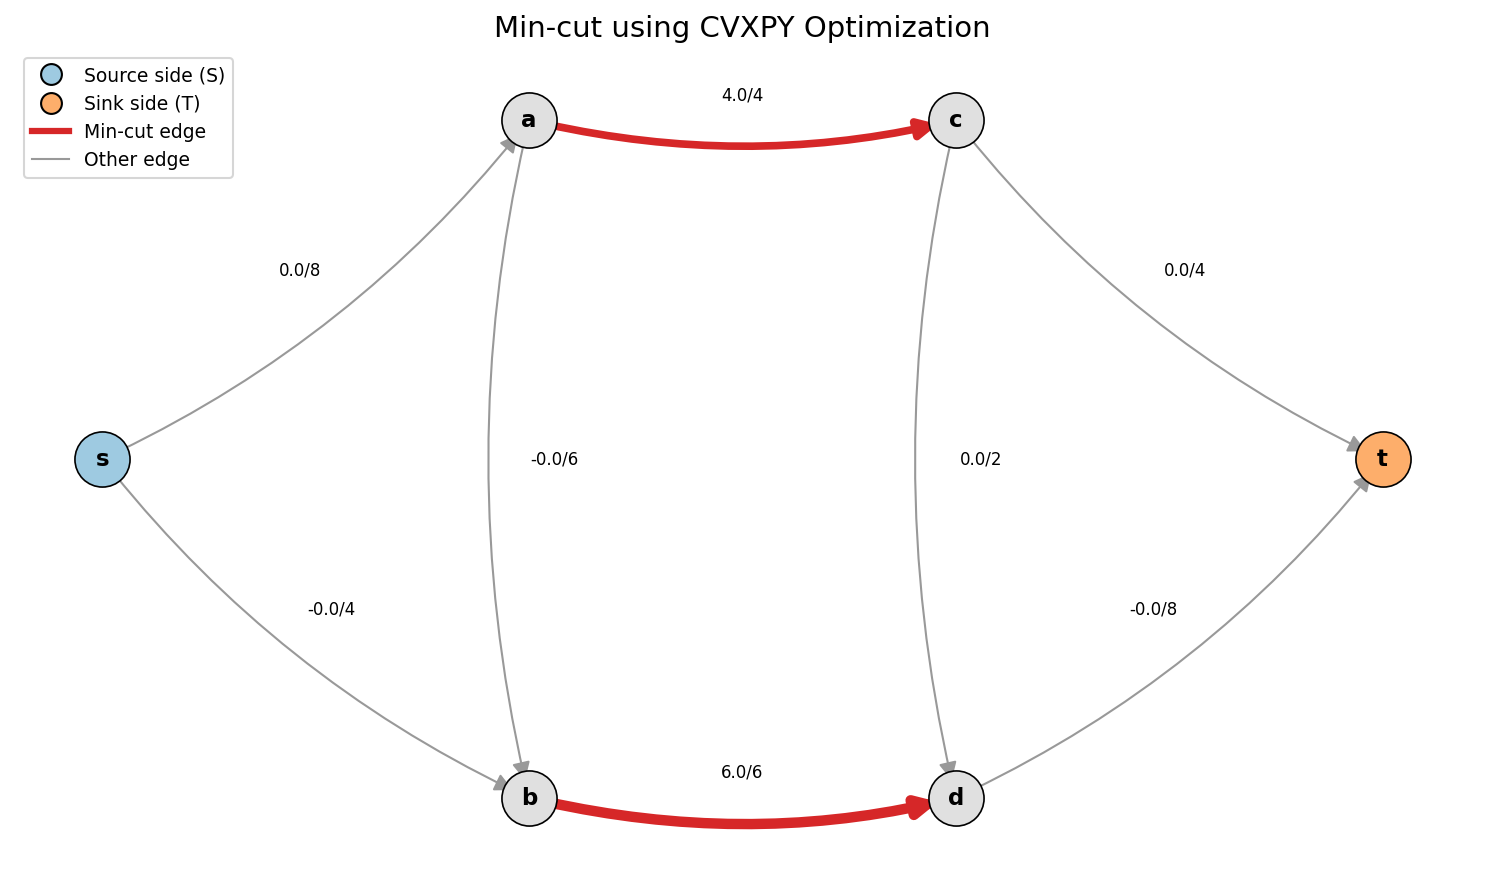
\includegraphics[width=\linewidth]{Project/img/cvxpy_min_cut.png}
        \caption{}
        \label{fig:cvxpy_min_cut}
    \end{subfigure}
    \caption{\textbf{Results of the Linear Program} The \figref{cvxpy_max_flow} presents edge utility saturation (\texttt{flow / capacity}. \figref{cvxpy_min_cut} highlights edges included in the cut, obtained by taking \texttt{d} edge variables vector to find the edges and multiplying them by \texttt{c} edge capacity vector to obtain the min-cut value}
    \label{fig:cvxpy_flow_network}
\end{figure}

\subsubsection{Algorithmic and LP results comparison}

Let us compare algorithmic and linear programming methods. In the case of Edmonds-Karp algorithm, the objective function of maximizing the flow wasn't specified by us - it is defined implicitly by the algorithm itself. The same holds true for the other flow algorithms included in the \texttt{networkx} package - maximization of the flow is implicit.

The interpretation of min-cut is also more straightforward - the algorithm terminated when there was no augmenting path from source to sink in the residual graph. The cut edges are the saturated edges crossing between two sets, that we found by using a graph searching algorithm that identified unreachable nodes in the residual graph, and thus, constitute a bottleneck limiting further increase of flow.

In contrast, the linear programming formulation describes the problem as general optimization problem with variables, constraints, and an explicit objective function. Linear programs do not exploit the combinatorial structure of the graph. This necessitated defining constraints for both problems separately, but as we will see, the differences don't end there.

The total flow values returned are identical, as both methods return optimal solution, but the edge flows differ. The "cleaner" appearance of the algorithmic approach is a result of the precise arithmetic nature of the combinatorial approach, while the observed values returned by LP originate from its numerical exploration of the real number space constrained by the linear equations, performed using floating point calculations.

The second difference is the necessity of defining constraints which are implicit in the flow algorithms. In the min-cut solution obtained using \texttt{cvxpy}, we can observe that the \(d\) and \(z\) vector variables contain values only in the \(\{0, 1\}\) range, which squares with our interpretation - edge can be either included or not, and the nodes potentials guarantee that edges connecting nodes of different sets are included in the cut. However, if we look at the defined constraints for the min-cut problem, \(z_u \in \mathbb{R}, d_{uv} \in \mathbb{R^+}\), allow them to take many real values outside of this range, and solutions which specify the edge inclusion as \(d_{uv} = 55.291...\) or \(d_{uv} = 0.5\) would be \textit{feasible}, even though conceptually, an edge can't be half-included in a cut. The question is, then, why do optimal solutions push those values towards the limits defined by other constraints.

Finally, we can see that despite the max-flow and min-cut optimization problems defining objective functions and many constraints separately, the resulting value is the same. This happens even though one is a maximization and the other a minimization problem. As we will demonstrate, this is a special example of strong duality - a pair of optimization problems, of which the value of optimal solution to one problem is equal to the other.

\subsection{Dual optimization and problem transformation}

Every linear optimization problem, which we will call \textit{primal}, can be used to derive a corresponding \textit{dual} problem. 
\begin{itemize}
    \item The variables in the primal correspond to constraints in the dual.
    \item The constraints in the primal become variables in the dual.
    \item The objective directions are reversed - when one is a maximization problem, the other is a minimization problem.
\end{itemize}

The primal problem creates a bound on the dual - for maximization, it is an upper bound. When the bounds are the same on both, then we can say that the \textit{duality gap} is equal to zero. We call this \textit{strong duality}. When there is a gap, it is a case of \textit{weak duality}.

The max-flow min-cut is a case of strong duality. Let us go through the process of deriving a dual in this example.

In general case

\[
\begin{aligned}
\text{Primal:} \qquad
\max \quad & c^\top x \\
\text{s.t.} \quad & Ax \le b, \\
& x \ge 0 .
\end{aligned}
\]

The respective dual is

\[
\begin{aligned}
\text{Dual:} \qquad
\min \quad & b^\top y \\
\text{s.t.} \quad & A^\top y \ge c, \\
& y \ge 0 .
\end{aligned}
\]

We can see that the primal constraint \(b\) now has a corresponding variable \(y\), and that the variable \(c\) became a constraint - now, it is used to define an upper bound that the dual minimizes.

Let us go through the process for max network flow problem

\[
\begin{aligned}
\text{Max-flow:} \qquad
\max \quad & q^\top x \\
\text{s.t.} \quad
& Ax = 0, \\
& 0 \le x \le c .
\end{aligned}
\]

To derive the dual formulation, we introduce dual variables corresponding to the constraints of the primal max-flow problem. The flow conservation constraint
\[
Ax = 0
\]
gives rise to the node-potential variables \(z\), while the capacity constraints
\[
x \le c
\]
give rise to the edge variables \(d\).

Thus, the primal--dual correspondence is
\[
\begin{aligned}
Ax = 0
&\quad \leftrightsquigarrow \quad z, \\
x \le c
&\quad \leftrightsquigarrow \quad d .
\end{aligned}
\]

Recall that \(A\) is the reduced node-edge incidence matrix, obtained by removing the rows corresponding to the source \(s\) and sink \(t\). Consequently, the vector \(A^\top z\) contains the potential differences between nonterminal nodes.

The dual problem can therefore be written compactly as
\[
\begin{aligned}
\text{minimize} \quad & d^\top c \\
\text{subject to} \quad
& d - A^\top z \ge q, \\
& d \ge 0 .
\end{aligned}
\]

Here, the vector \(q\) encodes the boundary conditions associated with the source and sink. In particular,
\[
q_i =
\begin{cases}
1, & \text{if } e_i=(s,v)\in E, \\[2pt]
0, & \text{otherwise.}
\end{cases}
\]

Because \(q\) already distinguishes edges leaving the source from all other edges, the dual constraints can be expressed uniformly in matrix form, without separately considering the cases \(u=s\) or \(v=t\). This revelation allowed us to simplify the python code that defines this problem, reducing 12 lines of code into 2.

\subsection{Lagrangian and Karush–Kuhn–Tucker conditions}\label{sec:lagrangian_kkt}

To explain how the primal and dual problems are connected, let us introduce the Lagrangian. The method of Lagrangian multipliers is a way of finding local maxima and minima of a function constrained by a set of equations.

For a standard problem

\[
\begin{aligned}
\text{Minimize} & \quad
f(x) \\[4pt]
\text{s.t} & \quad g_i(x)\le 0 \\[4pt]
&\quad  h_j(x)=0
\end{aligned}
\]

The Lagrangian function, or the \textit{Lagrangian}, generalized by the KKT conditions, is defined as

\begin{equation}
    \mathcal L(x,\lambda,\mu)=f(x)+\sum_i \lambda_i g_i(x)+\sum_j \mu_j h_j(x)
\end{equation}


Where \(\mu\) and \(\lambda\) are constants called the Lagrangian multipliers, or in this generalized form, \textit{KKT multipliers}.

In alternative form
\[ 
\alpha = \begin{bmatrix} \mu\\ \lambda\end{bmatrix}, \quad \mu \ge 0, 
\] 

\paragraph{Karush–Kuhn–Tucker theorem} 
\paragraph{Sufficiency} If \( (x^*, \alpha^*) \) is a saddle point of the Lagrangian \( L(x,\alpha)\) for \( x \in X, \quad \mu \ge 0 \), then \(x^*\) is an optimal solution of the optimization problem. 

\paragraph{Necessity} Suppose that \( f(x) \) and \( g_i(x), \quad i=1,\dots,m, \) are convex on \(X\), and that there exists \( x_0 \in \operatorname{relint}(X) \) such that \( g(x_0) < 0, \) that is, Slater's condition holds. Then for every optimal solution \(x^\ast\), there exists a vector 
\[ 
\alpha^\ast = \begin{bmatrix} \mu^\ast \\ \lambda^\ast \end{bmatrix}, \quad \mu^\ast \ge 0, 
\] 
such that \( (x^\ast,\alpha^\ast) \) is a saddle point of \( L(x,\alpha). \)

In plain language, sufficiency states that if a solution to a convex optimization problem, together with a set of multipliers, forms a saddle point of the Lagrangian, then the solution is optimal. In other words, the existence of a saddle point certifies optimality.

Conversely, necessity states that if a solution is optimal, then there exist multipliers such that the corresponding primal-dual pair forms a saddle point of the Lagrangian. Thus, under appropriate regularity conditions, every optimal primal solution has an associated dual solution that certifies its optimality.

\paragraph{Necessary conditions are:}
\begin{itemize}
\item Stationarity

Minimization:
\[
\partial f(x^*)+\sum_i \lambda_i^*\partial g_i(x^*)+\sum_j \mu_j^*\partial h_j(x^*) \ni 0
\]

Maximization:
\[
\partial f(x^*)-\sum_i \lambda_i^*\partial g_i(x^*)+\sum_j \mu_j^*\partial h_j(x^*) \ni 0
\]

\item Primal feasibility

\[
g_i(x^*)\le 0,\qquad \forall i
\]

\[
h_j(x^*)=0,\qquad \forall j
\]

\item Dual feasibility

\[
\lambda_i^*\ge 0,\qquad \forall i
\]

\[
\mu_j^* \in \mathbb{R},\qquad \forall j
\]

\item Complementary slackness

\[
\lambda_i^* g_i(x^*)=0,\qquad \forall i
\]
\end{itemize}

Now let us apply the conditions to maximum flow network problem. We have satisfied the \textit{Slater's regulary condition} by the way of \(x <  c\), that is, there exists a solution strictly satisfying all inequality conditions. Both objective function and the linear inequalities are convex.

We will represent the KKT conditions in matrix form.

\begin{itemize}
    \item \textbf{Stationarity} - for the maximization problem, the Lagrangian is
    \[
    L(x,d,z) = q^\top x + z^\top Ax + d^\top(c-x).
    \]

    Rearranging terms by \(x\),
    \[
    L(x,d,z) = d^\top c + (q + A^\top z - d)^\top x.
    \]

    Taking the gradient with respect to \(x\) yields the stationarity condition
    \[ 
    \nabla_x L(x,d,z) = q + A^\top z - d = 0.
    \]

    Equivalently,
    \[
    d - A^\top z = q.
    \]
    
    This should remind us of the min-cut inequality constraint,
    \[
    d - A^\top z \ge q.
    \]

    Indeed, this is an important insight into the dual problem. It shows that the edge variable $d$ is not arbitrary, that it has to balance the difference in node potentials $z$ on edges that exist in $A$. The minimum cut is not just a combinatorial partition of the graph, but also a balancing condition required by the optimality of maximum flow problem.


    \item \textbf{Primal feasibility}
    \[
    Ax = 0,
    \qquad
    0 \le x \le c.
    \]

    \item \textbf{Dual feasibility}
    \[
    d \ge 0.
    \]

    This is the source of the sign constraint of the min-cut problem. It guarantees that the edges don't cancel each other out when contributing to min-cut capacity objective, and thus ensuring the dual is truly a minimization problem.

    Moreover, this constrains node potentials $z$ by ensuring their values match the edge directions specified in the incidence matrix $A$.

    \item \textbf{Complementary slackness}
    \[
    d_i(c_i-x_i)=0,
    \qquad i=1,\dots,m.
    \]

    Thus, if an edge is not saturated (\(x_i<c_i\)), then \(d_i=0\); conversely, if \(d_i>0\), the edge capacity constraint is tight \(x_i = c_i\). Only fully saturated edges can be contained in the cut.

\end{itemize}

A final observation is that the vector \(q\) introduces a unit source-sink forcing through the constraints \(q_{su}=1\) for edges leaving the source. Through the stationarity condition, this forcing must propagate consistently across the graph via the node potentials

Combined with complementary slackness, the integral, unimodular structure of \(q\) and \(A\), this drives the optimal values of \(d_i\) toward either \(0\) or \(1\). Consequently, an edge either participates in separating the source from the sink, or it does not.


\subsection{Introducing fairness}

Previously, we have presented the allocation of resources throughout the network as a vector of flows:

\[
x = (x_1, x_2, \dots, x_n)
\]

In the maximum flow problem, the objective is the maximization of the total resource throughput. We may imagine the capacities as demands or supplies, and the flow as the utilization, or fulfillment of demands. The problem is abstract. In our basic case, the resource is a single, real-valued commodity, and the nodes could be seen as warehouses and hospitals, or as warehouses and regions.

The real resource allocation problem is much more complicated than that. In an epidemic outbreak, the total number of resources delivered, like the number of vaccines, masks or medical supplies distributed, is rarely the sole objective. In the real world, the problem may be extended to a multi-commodity, multi-objective, dynamic optimization or network planning problem, among others.

In this section, we will examine the concept of fairness as it relates to single real resource distribution - how to allocate it between edges so that no demand is starved, while still being efficient. Pure maximum flow problem may be useful when planning evacuation, where objective is to simply save as many people as possible, but in an epidemic outbreak scenario, if we imagine, for example, edges as hospitals with demand, we want to allocate resources like vaccines more evenly, so they can be distributed to the most vulnerable patients. This is just one scenario.


\paragraph{\textbf{Pareto Efficiency}} A solution is \textit{Pareto efficient} if you cannot improve one allocation without hurting another. Formally, allocation $x$ is Pareto efficient if there is no other feasible solution $y$ such that:

\[
y_i \ge x_i \quad \forall i
\]

and

\[
\exists\, j \in \{1,\dots,n\} \text{ such that } y_j > x_j.
\]

Which means every edge is at least as well off, and there is someone strictly better off. If such $y$ exists, then $x$ is not Pareto efficient.

\paragraph{\textbf{Pareto Frontier}} is a set of all Pareto efficient solutions. There may be many feasible solutions, and they form a feasible region, however, only the solutions on the "outer edge" of that region offer the best trade-offs.

As we have seen, LP solutions and Edmonds-Karp solutions to maximum flow problem differ, but both are Pareto efficient - flow on one edge cannot be improved without reducing flow on another edge.

The trade-offs between solution could have many definitions, like the flows on $e_i$ vs $e_j$, or trade-offs between optimization objectives, like total flow versus \textit{fairness}, however we define it, in our case.

The simple fact that a solution lies on a Pareto frontier does \textbf{not} make it fair. By defining an objective function, like the total flow \( \max f = \sum_{v \in V} f(s,v) \), we select the trade-off, and that can be interpreted as selecting a single point on a Pareto frontier. As we will see, we can define other objective functions to define different trade-offs.

\subsection{Types of fairness}
There are multitude of fairness objective definitions, but we will define two useful to us, and then generalize and approximate them in one, single parameter definition.

\paragraph{\textbf{Min-Max Fairness}} prioritizes the \textit{worst-off} edges. The goal is simple - improve the smallest allocations until no improvement can be made without decreasing flow of an edge with an equal or smaller allocation.

The standard way of computing min-max fairness is through \textit{progressive filling}. It progressively, iteratively increases utility like \(flow / capacity\) on edges until they reach they maximum allowable allocation. As it focuses on the worst-off allocations first, and makes it a basis for the second worst and so on, it can be viewed as a \textit{lexicographic} maximization method. We will not be implementing this algorithm, but we can approximate it.

\paragraph{Proportional Fairness}

Proportional fairness balances efficiency and fairness. Solution $x$ is proportionally fair if for any other feasible $y$ the sum of proportional gain is negative:
\[
\sum_i \frac{y_i - x_i}{x_i} \le 0
\]

The interpretation is that improvement for some edges causes larger proportional losses for others. The optimization utility to achieve such outcome is $\log(x)$, and the optimization objective:

\[
\max \sum_{(u,v)\in E}\log(x_{uv})
\]

For maximum flow objective, the marginal utility (how each unit is valued) is:
\[
\dv{}{x} x = 1
\]

So each added unit is valued equally. For log objective, the utility is valued:
\[
\dv{}{x} \log(x)=\frac{1}{x}
\]
Which is inversely proportional to the current allocation. Increasing flow has diminishing returns and should favor edges with small flows.

Another useful property of logarithms is:
\[
\log(ab)=\log a + \log b
\]

So maximizing sum of logs is equivalent to maximizing a product:

\[
\max \sum_i \log(x_i)
\quad\Longleftrightarrow\quad
\max \prod_i x_i
\]

This translates to the optimizer maximizing geometric mean instead of arithmetic mean. Geometric mean should penalize imbalance more.

\subsubsection{Alpha Fairness}
Alpha fairness is a family of fairness objectives that should unify our definitions:
\[
U_\alpha(x)=
\begin{cases}
\displaystyle \sum_i \frac{x_i^{1-\alpha}}{1-\alpha},
& \alpha \in [0,1)\cup(1,\infty) \\[1 em]
\displaystyle \sum_i \log(x_i),
& \alpha = 1
\end{cases}
\]
Note, that for $\alpha = 0$, the objective is a simple fairness-free total flow.

As for min-max fairness, the solution \(x^{\mathrm{MMF}}\) can be approximated with high $\alpha$, as shown in \cite{mo2000fair}:

\[
\lim_{\alpha \to \infty}
x^*(\alpha)
=
x^{\mathrm{MMF}}.
\]

This creates a unified definition of our fairness objectives, parametrized by a single parameter $\alpha$. The parameter $\alpha$ controls how much the objective penalises imbalance: $\alpha = 0$ ignores it entirely, $\alpha = 1$ gives proportional fairness, and $\alpha \to \infty$ maximises only the worst-off allocation. As we will demonstrate, $\alpha = 1$ is often the most appropriate choice under uniform conditions, and increasing $\alpha$ beyond this point can be counterproductive.

\subsection{Solving for fairness using convex optimization}

We have previously used Linear Programming formulations for max-flow and min-cut problems. In those cases, both objectives and constraints are linear. In order to solve nonlinear objectives such as $\log(x)$, we will use the closely related \textbf{convex optimization}. In truth, in our program nothing changes, because the optimizer used was already convex - all linear problems are also convex. This is a generalization of that idea which allows us to define more varied objectives.
 
\subsection{Cost of fairness - dual problem and shadow prices}


\subsection{Mathematical Framing and Theoretical Background}

We will use graph theory and the \textit{Max-Flow} problem to model our situation.

We will set an oriented graph $G=(V,E)$ where $V$ represents all the infrastructures (nodes) and $E$ the roads (edges). Each edge $(u,v)$ has a maximal capacity $c(u,v)$.

Our decision variable is $f(u,v)$, which represents the resources quantity on the edge $(u,v)$.

We will have three constraints \emph{Capacity constraint}, \emph{Flow conservation (Kirchhoff law)} and the flow value sign constraint
    \[
        f(u, v) \geq 0
    \]

Our objective function is therefore to maximize the total flow leaving the source $s$:

\begin{equation}
    \max f = \sum_{v \in V} f(s,v)
\end{equation}


The main theorem that we will use is the Max-Flow theorem (see \cite{dantzig1964maxflow} and \cite{wiki_maxflow_mincut}) in order to analyze the vulnerability of the network.

We will extend this model by using a "super-source" (connected to all usines) and a "super-well" (connected to all infected zone) in order to model a multi-cluster outbreak.

We will also define and use the sensibility of an edge $c$, which is the quantity $\frac{\Delta \abs{f}}{\Delta c_c}$ and we will try to find the most vital edge.


\section{Study of sensitivity}

\subsection{Context}

Based on the second presentation on the topic "Shortest path algorithms in weighted graphs", we used and improved the graph that represent Wrocław  city. The \figref{wroclaw_graph} presents the final graph that we will use to run our experiments.

In this graph, one can see the major position of the city such as the \textit{lotnisko}, fire station, the water plant or the hospital.

Regarding the capacity scale, we apply the following rules for the three types of categories:

\begin{itemize}
    \item weight of $50$ and more when it involves highways or major arteries such as the A4 or \textit{Legnicka};
    \item weight between $20$ and $40$ for standard city avenues such as the \textit{Plac Grunwaldzki};
    \item weight between $5$ and $15$ for the small streets, historic bridges and residential areas.
\end{itemize}

\begin{figure}[H]
    \centering
    
\includegraphics[width=0.9\linewidth]{img/wroclaw_graph.png}
    \caption{Wrocław graph used as a context for our work.}
    \label{fig:wroclaw_graph}
\end{figure}

\subsection{Sensitivity to capacity augmentation: duality and minimum cuts}\label{sec:partI}

Our goal is to \emph{identify the edges where increasing capacity improves overall throughput}, and those where it has no impact.

First, we will present the mathematical background to understand and solve this problem \ref{sec:1_theoretical_review}, then we will present a naive method to find those edges \ref{sec:1_naive_method}. Finally, we will present an optimized method based on a powerful mathematical result \ref{sec:1_optimized_method}.

\subsubsection{Theoretical review}\label{sec:1_theoretical_review}

The Max-Flow problem seeks to send the maximum amount of resources from a source $s$ to a sink $t$ in a directed graph $G=(V,E)$, where each edge $(i,j)$ has a maximum capacity $c_{ij}$.

Mathematically, we maximize the total flow $v$ subject to Kirchhoff's law \eqref{eq:kirchhoff_law} and the capacity constraint \eqref{eq:capacity_constraint}.

The Kirchhoff's law states that for any node $k \in V \backslash \{s,t\}$, the sum of incoming flows equals the sum of outgoing flows:

\begin{equation}\label{eq:kirchhoff_law}
    \sum_i f_{ik} - \sum_j f_{kj} = 0
\end{equation}

The capacity constraint states that we cannot exceed the capacity of each edge.

\begin{equation}\label{eq:capacity_constraint}
    \forall (i,j) \in E, \quad 0 \leq f_{ij} \leq c_{ij}
\end{equation}

The fundamental theorem states that the maximum flow is exactly equal to the capacity of the minimum cut (min-cut). A cut $(S,T)$ is a partition of the nodes such that $s \in S$ and $t\in T$. Its capacity is the sum of the capacities of the edges directed from $S$ to $T$.

If the capacity $c_{ij}$ of an edge is increased by a value $\delta$, the total flow $v$ will only increase if the edge $(i,j)$ belongs to the limiting minimum cut.

In terms of Linear Programming, sensitivity analysis corresponds to dual variables (or shadow prices). The dual variable associated with the capacity constraint $f_{ij} \leq c_{ij}$ indicates the marginal gain on the objective function (the flow) if this constraint is relaxed by one unit.

On the one hand, if the shadow price is strictly positive, the edge is a bottleneck (in the minimum cut). Increasing $c_{ij}$ increases the total flow. On the other hand, if the shadow price is zero, the edge's capacity is not saturated, or saturating it does not limit the overall flow. Increasing $c_{ij}$ is a waste of epidemiological resources.

\subsubsection{Naive method}\label{sec:1_naive_method}

First, the naive method can be considered: given a change $\delta$ on the edges capacity, we can for instance compute the total flow for every single edge of the graph and see if it improves the maximum flow.

\begin{python}[caption={Python code for the naive approach},  label={lst:1_naive_method_lst}]
def naive_sensitivity(G, s, t, delta=1):
    """
    Naive approach: Test every single edge to see if increasing its capacity improves the maximum flow.
    """
    base_flow_value = nx.maximum_flow_value(G, s, t)
    sensitivity_results = {}

    for u, v, data in G.edges(data=True):
        original_capacity = data['capacity']
        G[u][v]['capacity'] = original_capacity + delta
        
        new_flow_value = nx.maximum_flow_value(G, s, t)
        sensitivity_results[(u, v)] = new_flow_value - base_flow_value
        
        G[u][v]['capacity'] = original_capacity
        
    return sensitivity_results
\end{python}

\subsubsection{Optimized method}\label{sec:1_optimized_method}

However, the naive method is not optimal as we need to test every single edge. That is the reason why we can apply the \emph{Max-Flow Min-Cut Theorem} that states that if you increase the capacity $c_{ij}$ of and edge by a certain value $\delta$, the total flow will only increase if the edge belongs to the limiting minimum cut.

Therefore, we do not need to test every single edge, we only need to find and test the edges that are in limiting minimum cut. Hence, we are able to improve our method into an optimized method (\mylistref{1_optimized_method}).

\begin{python}[caption={Python code for the naive approach},  label={lst:1_optimized_method}]
def optimized_sensitivity(G, s, t, delta=1):
    """
    Optimized approach: Only test edges that cross the minimum s-t cut.
    """
    base_flow_value = nx.maximum_flow_value(G, s, t)
    sensitivity_results = { (u, v): 0 for u, v in G.edges() }
        
    # Find the minimum cut partition
    cut_value, partition = nx.minimum_cut(G, s, t)
    reachable, non_reachable = partition
    
    cut_edges = [(u, v) for u, v in G.edges() if u in reachable and v in non_reachable]
            
    for u, v in cut_edges:
        original_capacity = G[u][v]['capacity']
        G[u][v]['capacity'] = original_capacity + delta
        
        new_flow_value = nx.maximum_flow_value(G, s, t)
        sensitivity_results[(u, v)] = new_flow_value - base_flow_value
        
        G[u][v]['capacity'] = original_capacity
        
    return sensitivity_results
\end{python}

\subsubsection{Comparison and analysis}

As the naive method tests every single edge of the graph, by noting the total number of edges $\abs{E}$ (cardinal), this method requires exactly $1+\abs{E}$ number of iterations. However, the optimized method tests all edges within the min-cut (\tableref{nb_iterations_methods_1}).

\begin{table}[H]
    \centering
    \begin{tabular}{c | c}
         Method & Number of iterations \\
         \hline
         Naive & $1 + \abs{E}$\\
         Optimized & $1 + \abs{E_{\text{cut}}}$
    \end{tabular}
    \caption{Comparison of total number of iterations for each}
    \label{tab:nb_iterations_methods_1}
\end{table}

In order to compare these two methods, we will run a benchmark. First, we will generate a random Erdős-Rényi oriented graph and we will set a random capacity between $1$ and $15$. We make sure to check if there is a path from the source to the sink because, otherwise, the total flow is null and the test is not relevant.

Then we can track the evolution of computation time as a function of the size of the randomly generated graph (\figref{benchmark_1_all}). On the normal scale, we can see how efficient the optimized method is comparing to the naive method. As the graph's sizes are all in the same order of magnitude, the cardinal of the min-cut is similar which explains the low-growing function that we observe.

\begin{figure}[H]
    \centering
    \begin{subfigure}{.49\linewidth}
        \centering
        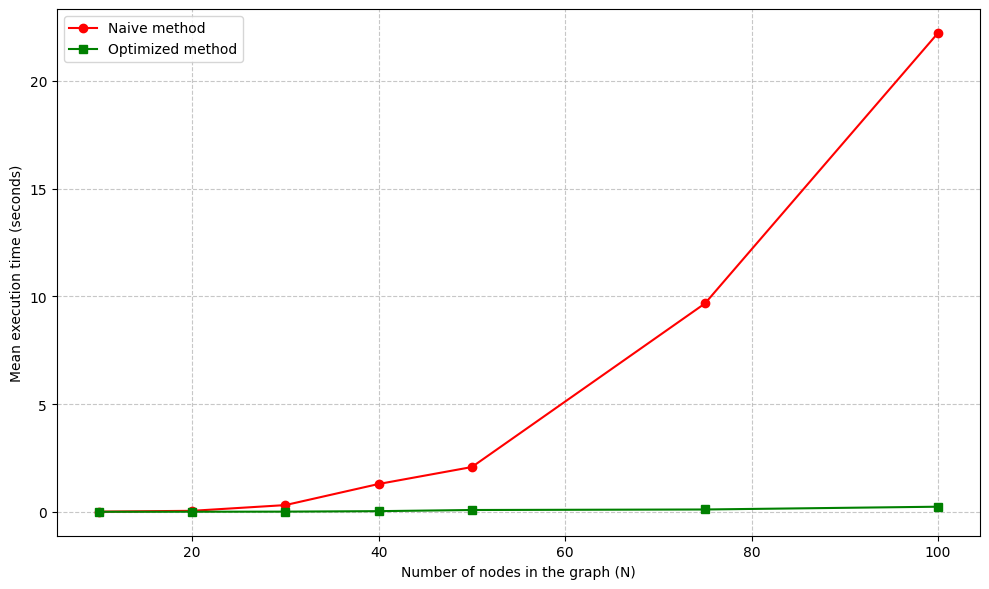
\includegraphics[width=\linewidth]{Project/img/benchmark_1.png}
        \caption{}
        \label{fig:benchmark_1}
    \end{subfigure}
    \begin{subfigure}{.49\linewidth}
        \centering
        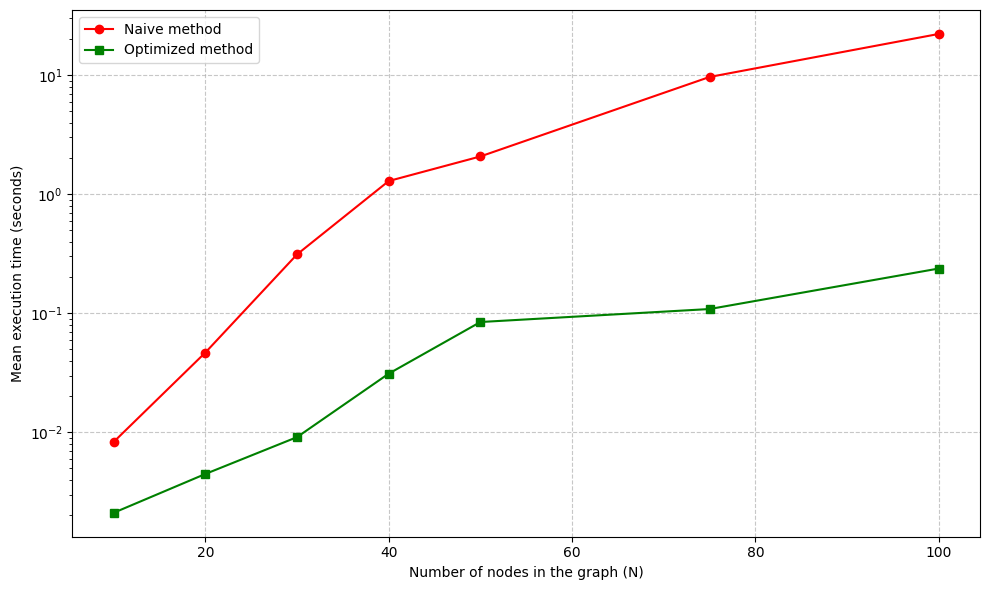
\includegraphics[width=\linewidth]{Project/img/benchmark_1_log.png}
        \caption{}
        \label{fig:benchmark_1_log}
    \end{subfigure}
    \caption{\textbf{Comparison between the naive and the optimized method.} \figref{benchmark_1} presents the performance with the number of nodes in the graph and \figref{benchmark_1_log} presents the same evolution using a $\log$ scale.}
    \label{fig:benchmark_1_all}
\end{figure}

This execution time comparison illustrates the computational overhead of recalculating flows and cuts, which further justifies avoiding iterative recalculation on large graphs, paving the way for the MILP formulation.

\subsubsection{Main observations}

Let us consider the graph in \figref{base_toy_graph_1}. We can see that the initial max flow is $11$. We observe that, if we add $+10$ to a non-bottleneck edge (between $S$ and $A$), then the new flow is also $11$. Therefore, adding capacity to a non-bottleneck edge is absolutely irrelevant.

Then, if we add $+10$ to a true bottleneck between node $A$ and $T$. Then, the new flow is $15$ so we have a gain of $+4$. What is the reason for that? In fact, the edge between node $S$ and $A$ became the \emph{new} bottleneck.

\begin{figure}[H]
    \centering
    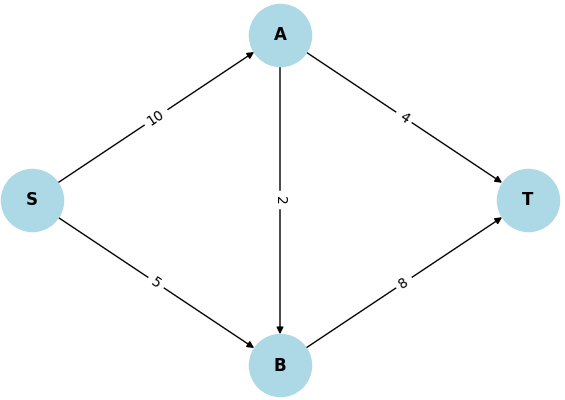
\includegraphics[width=0.5\linewidth]{Project/img/base_toy_graph_1.png}
    \caption{\textbf{Simple graph used to illustrate the case of a graph with multiple bottlenecks.}}
    \label{fig:base_toy_graph_1}
\end{figure}

Let us now consider the case where we have multiple min-cut edges. In order to study the impact on the total flow, let's consider the graph illustrated in \figref{base_toy_graph_2}.

The initial max flow is $10$ and we will upgrade one min cut (the edge between nodes $S$ and $A$) by $+5$. We observe then that the new flow is the same, the flow didn't increase because we are still constrained by the edge between $A$ and $T$.

We must therefore conclude that, in order to increase the flow, we need to upgrade systematically all simultaneous cuts.

\begin{figure}[H]
    \centering
    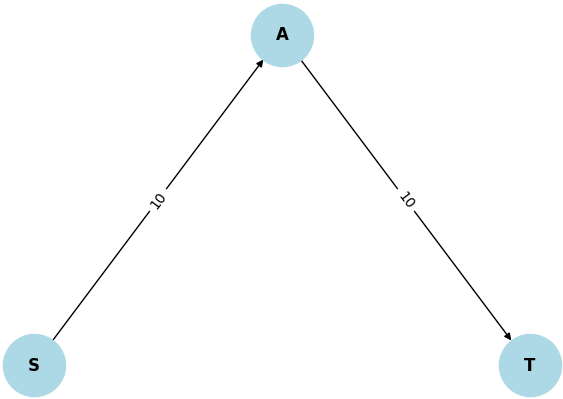
\includegraphics[width=0.5\linewidth]{Project/img/base_toy_graph_2.png}
    \caption{\textbf{Simple graph used to illustrate the need to upgrade all simultaneous cuts in order to increase the total flow.}}
    \label{fig:base_toy_graph_2}
\end{figure}

As demonstrated above, upgrading a single edge changes the entire bottleneck structure of the network. Because the number of possible cuts grows exponentially ($O(2^n)$), calculating all min-cuts to decide on multiple upgrades is highly inefficient. Furthermore, a Greedy approach fails here because an irrevocable upgrade choice in one iteration might lead to sub-optimal bottlenecks in the next. This proves that assigning a multi-edge budget is a complex Combinatorial / NP-hard problem.

\subsection{Identification of the most critical edge}

Our goal is now to measure the flow loss if an edge is completely removed (or if its capacity is reduced to zero). This can be the case if, for instance, a road is removed or if an unexpected issue occurs.

First, we will present the mathematical background to understand and solve this problem \ref{sec:2_theoretical_review}, then we will present a naive method to find those edges \ref{sec:2_naive_method}. Finally, we will present a optimized method based on a powerful mathematical result \ref{sec:2_optimized_method}.

\subsubsection{Theoretical review}\label{sec:2_theoretical_review}

Here, we are no longer looking at expansion, but at the resilience of the network (e.g., what happens if a route is cut off by floods or if a warehouse fails?).

We define the "vitality" of an edge $e$ by the decrease in the maximum flow value $\Delta v(e)$ when this edge is removed from the network:

\begin{equation}
    \Delta v(e) = \abs{f}_{max}(G) - \abs{f}_{max}\left(G \backslash\{e\}\right)
\end{equation}

We will explore the mathematical properties of this quantity.

First, as the the flow loss cannot exceed the capacity of the removed edge, nor the actual flow passing through it, we can provide an upper bound \eqref{eq:upper_bound}.

\begin{equation}\label{eq:upper_bound}
    \Delta v(e) \leq f(e) \leq c(e)
\end{equation}

Then, we can discuss the connection of the vitality with the minimum cut. An edge $e$ has a vitality $\Delta v(e) > 0$ \textit{if and only if} it belongs to all possible minimum cuts of the graph. If it only belongs to some minimum cuts, the flow can find another path that will saturate an alternative cut, and the loss will be strictly less than $c(e)$.

The comparison is indeed why the identification of the minimum cut edges is an excellent pre-selection heuristic to significantly reduce computational time (TO DEVELOPP).

\subsubsection{Naive method}\label{sec:2_naive_method}

First, the naive method can be considered: for every single edge in the graph, we can simulate his removal, compute the final total flow and save it. At the end, we return the edge that causes the maximum flow loss.

\begin{python}[caption={Python code for the naive approach in order to identify the most vital edge},  label={lst:2_naive_method_lst}]
def find_most_vital_edge_naive(G, s, t):
    """
    Identifies the 'most vital edge' in a flow network.
    The most vital edge is the one whose removal causes the largest decrease in the maximum flow.
    """
    base_flow_value = nx.maximum_flow_value(G, s, t)
    
    most_vital_edge = None
    max_flow_loss = -1
    edge_losses = {}
    
    for u, v, data in G.edges(data=True):
        original_capacity = data['capacity']
        if original_capacity == 0: continue
            
        # Simulate edge removal
        G[u][v]['capacity'] = 0
        new_flow_value = nx.maximum_flow_value(G, s, t)
        
        flow_loss = base_flow_value - new_flow_value
        edge_losses[(u, v)] = flow_loss
        
        if flow_loss > max_flow_loss:
            max_flow_loss = flow_loss
            most_vital_edge = (u, v)
            
        G[u][v]['capacity'] = original_capacity
        
    return most_vital_edge, max_flow_loss, edge_losses
\end{python}

\subsubsection{Optimized method}\label{sec:2_optimized_method}

In fact, if the edge has no flow, his loss will be $0$. We can therefore save all these edges and avoid useless computation.

\begin{python}[caption={Python code for the naive approach in order to identify the most vital edge},  label={lst:2_naive_method_lst}]
def find_most_vital_edge_optimized(G, s, t):
    # compute the flow and recuperation of the flow distribution
    base_flow_value, flow_dict = nx.maximum_flow(G, s, t)
    
    most_vital_edge = None
    max_flow_loss = -1
    edge_losses = {} # dict to save all the losses
    
    for u, v, data in G.edges(data=True):
        original_capacity = data['capacity']
        
        # ignore the edges that haven't any capacity
        if original_capacity == 0: 
            edge_losses[(u, v)] = 0
            continue
            
        # optimization here
        # if the edge hasn't flow, his loss is 0
        # we save it to the dict and we do not compute again the total flow
        if flow_dict[u].get(v, 0) == 0:
            edge_losses[(u, v)] = 0
            continue
            
        # simulation of the releting only for active edges
        G[u][v]['capacity'] = 0
        new_flow_value = nx.maximum_flow_value(G, s, t)
        
        flow_loss = base_flow_value - new_flow_value
        edge_losses[(u, v)] = flow_loss
        
        if flow_loss > max_flow_loss:
            max_flow_loss = flow_loss
            most_vital_edge = (u, v)
            
        # restoration of the original capacity
        G[u][v]['capacity'] = original_capacity
        
    return most_vital_edge, max_flow_loss, edge_losses
\end{python}

\subsubsection{Comparison and analysis}

In order to compare these two methods, we will run the same benchmark.
Then we can track the evolution of computation time in function of the size of the random generated graph (\figref{benchmark_2_all}). On the normal scale, we can see how efficient the optimized method is comparing to the naive method. As the graph's size are all in the same order, the cardinal of the min-cut is similar which explains the low-growing function that we observe.

\begin{figure}[H]
    \centering
    \begin{subfigure}{.49\linewidth}
        \centering
        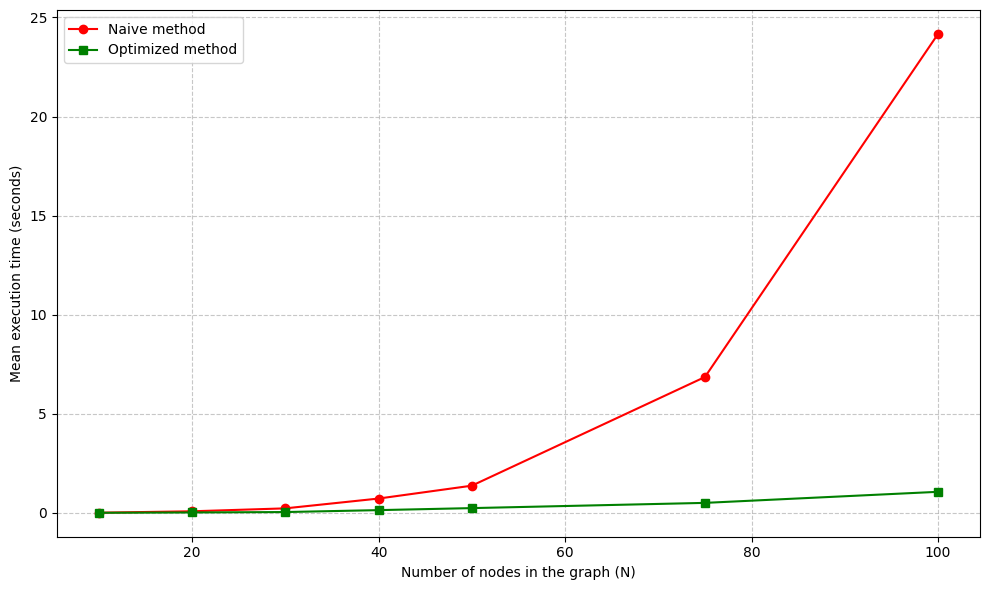
\includegraphics[width=\linewidth]{Project/img/benchmark_2.png}
        \caption{}
        \label{fig:benchmark_2}
    \end{subfigure}
    \begin{subfigure}{.49\linewidth}
        \centering
        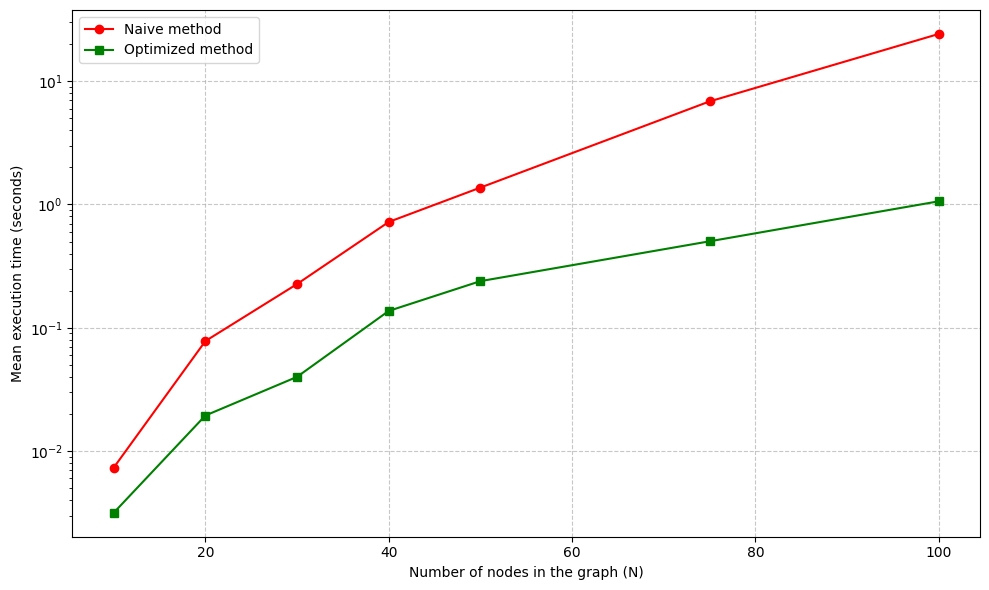
\includegraphics[width=\linewidth]{Project/img/benchmark_2_log.png}
        \caption{}
        \label{fig:benchmark_2_log}
    \end{subfigure}
    \caption{\textbf{Comparison between the naive and the optimized method.} The \figref{benchmark_2} present the performance with the number of nodes in the graph and the \figref{benchmark_2_log} present the same evolution using a $\log$ scale.}
    \label{fig:benchmark_2_all}
\end{figure}

\subsection{Optimal sequence of $k$ edges subject to a budget constraint}

In section \ref{sec:partI}, we established that a greedy edge-by-edge upgrade strategy is mathematically flawed for holistic network planning. Therefore, to find the true optimal combination of upgrades within a set budget, we must use Mixed-Integer Linear Programming (MILP) which evaluates the entire search tree globally rather than myopically.


\subsubsection{Theoretical review}

We transition from a simple analysis problem to a Network Design Problem, where we have a certain budget $B$. Increasing the capacity of an edge $(i,j)$ by one unit costs $w_{ij}$. We introduce a new decision variable $y_{ij} \geq 0$ representing the added capacity.

The new linear program becomes therefore to maximize $v$ under the following constraints:

\begin{equation}
    \begin{cases}
        \forall k \in V \backslash \{s,t\}, \quad \sum_i f_{ik} - \sum_j f_{kj} = 0 \qquad &\text{(Kirchoff's law)} \\
        \forall (i,j) \in E, \quad 0 \leq f_{ij} \leq c_{ij} + y_{ij} \qquad &\text{(Capacity's constraint)} \\
        \sum_{(i,j) \in E} w_{ij} y_{ij} \leq B \qquad &\text{(Budget's constraint)} \\
    \end{cases}
\end{equation}

\subsubsection{Greedy algorithm}

The greedy method aims to iteratively select the best single edge to upgrade (\mylistref{3_greedy_method_lst}).

\begin{python}[caption={Python code for the greedy approach in order to identify the sequence of $k$ edges under budget constraint},  label={lst:3_greedy_method_lst}]
def greedy_k_edges(G, s, t, k, delta=1.0):
    """Greedy approach: Iteratively selects the best single edge to upgrade."""
    G_temp = G.copy()
    chosen_edges = []
    
    for i in range(k):
        best_edge, max_gain = None, 0
        base_flow = nx.maximum_flow_value(G_temp, s, t)
        
        for u, v in G_temp.edges():
            G_temp[u][v]['capacity'] += delta
            gain = nx.maximum_flow_value(G_temp, s, t) - base_flow
            
            if gain > max_gain:
                max_gain = gain
                best_edge = (u, v)
                
            G_temp[u][v]['capacity'] -= delta
            
        if best_edge:
            chosen_edges.append(best_edge)
            G_temp[best_edge[0]][best_edge[1]]['capacity'] += delta
        else:
            break
            
    return chosen_edges, nx.maximum_flow_value(G_temp, s, t)


\end{python}

However, the greedy algorithm is not always optimal because the maximum flow function is not strictly submodular with respect to capacity addition.

In discrete mathematics, a greedy algorithm offers strong approximation guarantees if the objective function exhibits diminishing marginal returns (submodularity). However, in a network, increasing the capacity of route A might yield zero gain until you also increase the capacity of the subsequent route $B$ (synergy effect). The greedy approach will ignore $A$ and B because their immediate individual gain is $0$, whereas the joint investment in $(A + B)$ would have been the global optimum.

\subsubsection{Linear Programming}

The LP Solver (implemented in pulp module), by evaluating the solution space holistically (using the simplex algorithm or interior point methods), will capture this synergy that the greedy algorithm misses (\mylistref{3_ilp_method_lst}).

\begin{python}[caption={Python code for the greedy approach in order to identify the sequence of $k$ edges under budget constraint},  label={lst:3_ilp_method_lst}]
def exact_k_edges_ilp(G, s, t, k, delta=1.0):
    """Exact approach using Mixed Integer Linear Programming (MILP)."""
    prob = pulp.LpProblem("Max_Flow_Budget", pulp.LpMaximize)
    flows, upgrades = {}, {}
    
    for u, v in G.edges():
        flows[(u, v)] = pulp.LpVariable(f"flow_{u}_{v}", lowBound=0)
        upgrades[(u, v)] = pulp.LpVariable(f"up_{u}_{v}", cat=pulp.LpBinary)
        
    prob += pulp.lpSum([flows[(s, v)] for v in G.successors(s)]), "Total_Flow"
    prob += pulp.lpSum(upgrades.values()) <= k, "Budget"
    
    for u, v, data in G.edges(data=True):
        base_cap = data['capacity']
        prob += flows[(u, v)] <= base_cap + (upgrades[(u, v)] * delta)
        
    for node in G.nodes():
        if node not in [s, t]:
            prob += pulp.lpSum([flows[(u, node)] for u in G.predecessors(node)]) == \
                    pulp.lpSum([flows[(node, v)] for v in G.successors(node)])
            
    prob.solve(pulp.PULP_CBC_CMD(msg=False))
    
    chosen_edges = [(u, v) for u, v in G.edges() if pulp.value(upgrades[(u, v)]) > 0.5]
    return chosen_edges, pulp.value(prob.objective)
\end{python}

\subsubsection{Comparison and analysis}

Finally, we will continue to use generated random graph to compare both methods. On the one hand, we can follow the evolution of the computational time with the size of the graph (\figref{benchmark_3a}). On the other hand, we can study how the greedy method is in fact close to the optimal solution (\figref{benchmark_3b}).

\begin{figure}[H]
    \centering
    \begin{subfigure}{.49\linewidth}
        \centering
        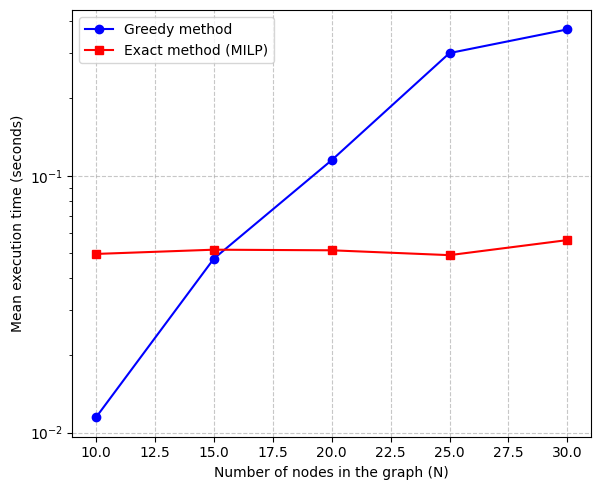
\includegraphics[width=\linewidth]{Project/img/benchmark_3a.png}
        \caption{}
        \label{fig:benchmark_3a}
    \end{subfigure}
    \begin{subfigure}{.49\linewidth}
        \centering
        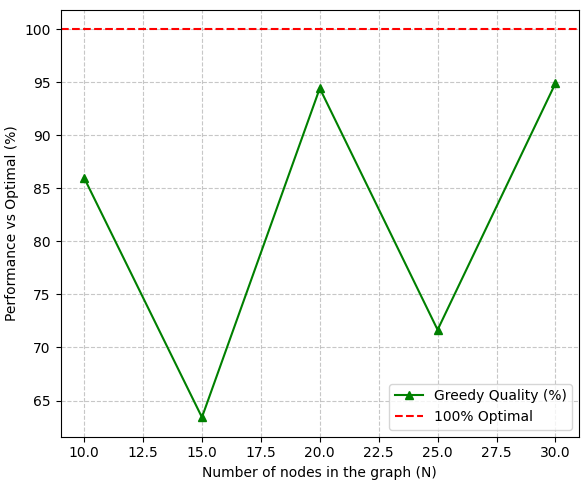
\includegraphics[width=\linewidth]{Project/img/benchmark_3b.png}
        \caption{}
        \label{fig:benchmark_3b}
    \end{subfigure}
    \caption{\textbf{Comparison between the greedy and the linear programming.} \figref{benchmark_3a} presents the execution time with the number of nodes in the graph and \figref{benchmark_3b} presents efficiency of the greedy algorithm comparing with the real optimal solution.}
    \label{fig:benchmark_3}
\end{figure}

\section{Further development (as homework ?)}

\addcontentsline{toc}{section}{Conclusion}
\section*{Conclusion}

\addcontentsline{toc}{section}{References}
\section*{References}
\printbibliography[sorting=nyt, heading=none]

\newpage
\addcontentsline{toc}{section}{Appendixes}
\section*{Appendixes}


\addcontentsline{toc}{subsection}{List of Tables}

\listoftables

\addcontentsline{toc}{subsection}{List of Figures}

\listoffigures

\addcontentsline{toc}{subsection}{List of Algorithms}

\listofalgorithms

\addcontentsline{toc}{subsection}{List of Listings}

\lstlistoflistings

\end{document} 